%\documentclass[10pt,handout]{beamer}
\documentclass[10pt]{beamer}
\usepackage[english]{babel} % Anpassa efter svenska. Ger svensk logga.
\usepackage[utf8]{inputenc} % Anpassa efter linux
\usepackage{graphicx}
\usepackage{hyperref}
\usepackage{listings}
\lstdefinelanguage{Stan}{
  morekeywords=[1]{functions,data,parameters,transformed,model,generated,quantities,%
    for,in,while,print,if,else,lower,upper,increment_log_prob,T,return,%
    reject,integrate_ode,integrate_ode_bdf,integrate_ode_rk45,target},%
  morekeywords=[2]{int,real,vector,%
    ordered,positive_ordered,simplex,unit_vector,%
    row_vector,matrix,%
    cholesky_factor_corr,cholesky_factor_cov,%
    coor_matrix,cov_matrix,%
    void},%
  morekeywords=[3]{%
    Phi,%
    Phi_approx,%
    abs,%
    acos,%
    acosh,%
    append_col,%
    append_row,%
    asin,%
    asinh,%
    atan,%
    atan2,%
    atanh,%
    bernoulli_cdf,%
    bernoulli_cdf_log,%
    bernoulli_lccdf,%
    bernoulli_lcdf,%
    bernoulli_logit_lpmf,%
    bernoulli_logit_lpmf,%
    bernoulli_lpmf,%
    bernoulli_lpmf,%
    bernoulli_rng,%
    bessel_first_kind,%
    bessel_second_kind,%
    beta_binomial_cdf,%
    beta_binomial_cdf_log,%
    beta_binomial_lccdf,%
    beta_binomial_lcdf,%
    beta_binomial_lpmf,%
    beta_binomial_lpmf,%
    beta_binomial_rng,%
    beta_cdf,%
    beta_cdf_log,%
    beta_lccdf,%
    beta_lcdf,%
    beta_lpdf,%
    beta_lpdf,%
    beta_rng,%
    binary_log_loss,%
    binomial_cdf,%
    binomial_cdf_log,%
    binomial_coefficient_log,%
    binomial_lccdf,%
    binomial_lcdf,%
    binomial_logit_lpmf,%
    binomial_logit_lpmf,%
    binomial_lpmf,%
    binomial_lpmf,%
    binomial_rng,%
    block,%
    categorical_logit_lpmf,%
    categorical_logit_lpmf,%
    categorical_lpmf,%
    categorical_lpmf,%
    categorical_rng,%
    cauchy_cdf,%
    cauchy_cdf_log,%
    cauchy_lccdf,%
    cauchy_lcdf,%
    cauchy_lpdf,%
    cauchy_lpdf,%
    cauchy_rng,%
    cbrt,%
    ceil,%
    chi_square_cdf,%
    chi_square_cdf_log,%
    chi_square_lccdf,%
    chi_square_lcdf,%
    chi_square_lpdf,%
    chi_square_lpdf,%
    chi_square_rng,%
    cholesky_decompose,%
    col,%
    cols,%
    columns_dot_product,%
    columns_dot_self,%
    cos,%
    cosh,%
    crossprod,%
    csr_extract_u,%
    csr_extract_v,%
    csr_extract_w,%
    csr_matrix_times_vector,%
    csr_to_dense_matrix,%
    cumulative_sum,%
    determinant,%
    diag_matrix,%
    diag_post_multiply,%
    diag_pre_multiply,%
    diagonal,%
    digamma,%
    dims,%
    dirichlet_lpdf,%
    dirichlet_lpdf,%
    dirichlet_rng,%
    distance,%
    dot_product,%
    dot_self,%
    double_exponential_cdf,%
    double_exponential_cdf_log,%
    double_exponential_lccdf,%
    double_exponential_lcdf,%
    double_exponential_lpdf,%
    double_exponential_lpdf,%
    double_exponential_rng,%
    e,%
    eigenvalues_sym,%
    eigenvectors_sym,%
    erf,%
    erfc,%
    exp,%
    exp2,%
    exp_mod_normal_cdf,%
    exp_mod_normal_cdf_log,%
    exp_mod_normal_lccdf,%
    exp_mod_normal_lcdf,%
    exp_mod_normal_lpdf,%
    exp_mod_normal_lpdf,%
    exp_mod_normal_rng,%
    expm1,%
    exponential_cdf,%
    exponential_cdf_log,%
    exponential_lccdf,%
    exponential_lcdf,%
    exponential_lpdf,%
    exponential_lpdf,%
    exponential_rng,%
    fabs,%
    falling_factorial,%
    fdim,%
    floor,%
    fma,%
    fmax,%
    fmin,%
    fmod,%
    frechet_cdf,%
    frechet_cdf_log,%
    frechet_lccdf,%
    frechet_lcdf,%
    frechet_lpdf,%
    frechet_lpdf,%
    frechet_rng,%
    gamma_cdf,%
    gamma_cdf_log,%
    gamma_lccdf,%
    gamma_lcdf,%
    gamma_lpdf,%
    gamma_lpdf,%
    gamma_p,%
    gamma_q,%
    gamma_rng,%
    gaussian_dlm_obs_lpdf,%
    gaussian_dlm_obs_lpdf,%
    get_lp,%
    gumbel_cdf,%
    gumbel_cdf_log,%
    gumbel_lccdf,%
    gumbel_lcdf,%
    gumbel_lpdf,%
    gumbel_lpdf,%
    gumbel_rng,%
    head,%
    hypergeometric_lpmf,%
    hypergeometric_lpmf,%
    hypergeometric_rng,%
    hypot,%
    if_else,%
    inc_beta,%
    int_step,%
    inv,%
    inv_chi_square_cdf,%
    inv_chi_square_cdf_log,%
    inv_chi_square_lccdf,%
    inv_chi_square_lcdf,%
    inv_chi_square_lpdf,%
    inv_chi_square_lpdf,%
    inv_chi_square_rng,%
    inv_cloglog,%
    inv_gamma_cdf,%
    inv_gamma_cdf_log,%
    inv_gamma_lccdf,%
    inv_gamma_lcdf,%
    inv_gamma_lpdf,%
    inv_gamma_lpdf,%
    inv_gamma_rng,%
    inv_logit,%
    inv_phi,%
    inv_sqrt,%
    inv_square,%
    inv_wishart_lpdf,%
    inv_wishart_lpdf,%
    inv_wishart_rng,%
    inverse,%
    inverse_spd,%
    is_inf,%
    is_nan,%
    lbeta,%
    lchoose,%
    lgamma,%
    lkj_corr_cholesky_lpdf,%
    lkj_corr_cholesky_lpdf,%
    lkj_corr_cholesky_rng,%
    lkj_corr_lpdf,%
    lkj_corr_lpdf,%
    lkj_corr_rng,%
    lmgamma,%
    lmultiply,%
    log,%
    log10,%
    log1m,%
    log1m_exp,%
    log1m_inv_logit,%
    log1p,%
    log1p_exp,%
    log2,%
    log_determinant,%
    log_diff_exp,%
    log_falling_factorial,%
    log_inv_logit,%
    log_mix,%
    log_rising_factorial,%
    log_softmax,%
    log_sum_exp,%
    logistic_cdf,%
    logistic_cdf_log,%
    logistic_lccdf,%
    logistic_lcdf,%
    logistic_lpdf,%
    logistic_lpdf,%
    logistic_rng,%
    logit,%
    lognormal_cdf,%
    lognormal_cdf_log,%
    lognormal_lccdf,%
    lognormal_lcdf,%
    lognormal_lpdf,%
    lognormal_lpdf,%
    lognormal_rng,%
    machine_precision,%
    max,%
    mdivide_left_tri_low,%
    mdivide_right_tri_low,%
    mean,%
    min,%
    modified_bessel_first_kind,%
    modified_bessel_second_kind,%
    multi_gp_cholesky_lpdf,%
    multi_gp_cholesky_lpdf,%
    multi_gp_lpdf,%
    multi_gp_lpdf,%
    multi_normal_cholesky_lpdf,%
    multi_normal_cholesky_lpdf,%
    multi_normal_cholesky_rng,%
    multi_normal_lpdf,%
    multi_normal_lpdf,%
    multi_normal_prec_lpdf,%
    multi_normal_prec_lpdf,%
    multi_normal_rng,%
    multi_student_t_lpdf,%
    multi_student_t_lpdf,%
    multi_student_t_rng,%
    multinomial_lpmf,%
    multinomial_lpmf,%
    multinomial_rng,%
    multiply_log,%
    multiply_lower_tri_self_transpose,%
    neg_binomial_2_cdf,%
    neg_binomial_2_cdf_log,%
    neg_binomial_2_lccdf,%
    neg_binomial_2_lcdf,%
    neg_binomial_2_log_lpmf,%
    neg_binomial_2_log_lpmf,%
    neg_binomial_2_log_rng,%
    neg_binomial_2_lpmf,%
    neg_binomial_2_lpmf,%
    neg_binomial_2_rng,%
    neg_binomial_cdf,%
    neg_binomial_cdf_log,%
    neg_binomial_lccdf,%
    neg_binomial_lcdf,%
    neg_binomial_lpmf,%
    neg_binomial_lpmf,%
    neg_binomial_rng,%
    negative_infinity,%
    normal_cdf,%
    normal_cdf_log,%
    normal_lccdf,%
    normal_lcdf,%
    normal_lpdf,%
    normal_lpdf,%
    normal_rng,%
    not_a_number,%
    num_elements,%
    ordered_logistic_lpmf,%
    ordered_logistic_lpmf,%
    ordered_logistic_rng,%
    owens_t,%
    pareto_cdf,%
    pareto_cdf_log,%
    pareto_lccdf,%
    pareto_lcdf,%
    pareto_lpdf,%
    pareto_lpdf,%
    pareto_rng,%
    pareto_type_2_cdf,%
    pareto_type_2_cdf_log,%
    pareto_type_2_lccdf,%
    pareto_type_2_lcdf,%
    pareto_type_2_lpdf,%
    pareto_type_2_lpdf,%
    pareto_type_2_rng,%
    pi,%
    poisson_cdf,%
    poisson_cdf_log,%
    poisson_lccdf,%
    poisson_lcdf,%
    poisson_log_lpmf,%
    poisson_log_lpmf,%
    poisson_log_rng,%
    poisson_lpmf,%
    poisson_lpmf,%
    poisson_rng,%
    positive_infinity,%
    pow,%
    prod,%
    qr_Q,%
    qr_R,%
    quad_form,%
    quad_form_diag,%
    quad_form_sym,%
    rank,%
    rayleigh_cdf,%
    rayleigh_cdf_log,%
    rayleigh_lccdf,%
    rayleigh_lcdf,%
    rayleigh_lpdf,%
    rayleigh_lpdf,%
    rayleigh_rng,%
    rep_array,%
    rep_matrix,%
    rep_row_vector,%
    rep_vector,%
    rising_factorial,%
    round,%
    row,%
    rows,%
    rows_dot_product,%
    rows_dot_self,%
    scaled_inv_chi_square_cdf,%
    scaled_inv_chi_square_cdf_log,%
    scaled_inv_chi_square_lccdf,%
    scaled_inv_chi_square_lcdf,%
    scaled_inv_chi_square_lpdf,%
    scaled_inv_chi_square_lpdf,%
    scaled_inv_chi_square_rng,%
    sd,%
    segment,%
    sin,%
    singular_values,%
    sinh,%
    size,%
    skew_normal_cdf,%
    skew_normal_cdf_log,%
    skew_normal_lccdf,%
    skew_normal_lcdf,%
    skew_normal_lpdf,%
    skew_normal_lpdf,%
    skew_normal_rng,%
    softmax,%
    sort_asc,%
    sort_desc,%
    sort_indices_asc,%
    sort_indices_desc,%
    sqrt,%
    sqrt2,%
    square,%
    squared_distance,%
    step,%
    student_t_cdf,%
    student_t_cdf_log,%
    student_t_lccdf,%
    student_t_lcdf,%
    student_t_lpdf,%
    student_t_lpdf,%
    student_t_rng,%
    sub_col,%
    sub_row,%
    sum,%
    tail,%
    tan,%
    tanh,%
    tcrossprod,%
    tgamma,%
    to_array_1d,%
    to_array_2d,%
    to_matrix,%
    to_row_vector,%
    to_vector,%
    trace,%
    trace_gen_quad_form,%
    trace_quad_form,%
    trigamma,%
    trunc,%
    uniform_cdf,%
    uniform_cdf_log,%
    uniform_lccdf,%
    uniform_lcdf,%
    uniform_lpdf,%
    uniform_lpdf,%
    uniform_rng,%
    variance,%
    von_mises_lpdf,%
    von_mises_lpdf,%
    von_mises_rng,%
    weibull_cdf,%
    weibull_cdf_log,%
    weibull_lccdf,%
    weibull_lcdf,%
    weibull_lpdf,%
    weibull_lpdf,%
    weibull_rng,%
    wiener_lpdf,%
    wiener_lpdf,%
    wishart_lpdf,%
    wishart_lpdf,%
    wishart_rng
  },%
  otherkeywords={<-,~,+=,=},%
  sensitive=true,%
  morecomment=[l]{\#},%
  morecomment=[l]{//},%
  morecomment=[n]{/*}{*/},%
  string=[d]"%,
  literate={<-}{{$\leftarrow$}}1 {~}{{$\sim$}}1%
}
 % Stan listing[language=Stan]

\hypersetup{
    colorlinks=true,
    linkcolor=blue,
    filecolor=magenta,
    urlcolor=cyan,
}
\usepackage{../common/beamerthemeUppsala}
%\usetheme{Uppsala}
%\usecolortheme{UU} % Anpassa efter UU:s frger och logga
%\hypersetup{pdfpagemode=FullScreen} % Adobe Reader ska ppna fullskrm
\setbeamertemplate{itemize items}[circle]

% \usepackage{beamerthemesplit}
\usepackage{amsmath}
% \usepackage{amssymb}
% \usepackage{graphics}
% \usepackage{graphicx}
% \usepackage{epsfig}
% \usepackage[latin1]{inputenc}
 \usepackage{color}
% \usepackage{fancybox}
% \usepackage{psfrag}
% \usepackage[english]{babel}
 \setbeamertemplate{footline}{\hfill\insertframenumber/\inserttotalframenumber}

% Input new commands
%\usepackage{bm}
%\usepackage{natbib}
\newcommand{\bfm}[1]   {\mbox{\boldmath{${#1}$}}}
\newcommand{\Prob}   {\mbox{\textnormal{P}}}
\def\eqd{\,{\buildrel d \over =}\,}

% Vector/Matrix definitions (in bold type)
\newcommand{\vect}[1]{\mathbf{#1}}
\newcommand{\vectb}[1]{\bm{#1}}

% Differential operator 'd' as upright as in (use \dd)
\newcommand{\dd}{\; \mathrm{d}}

% Gaussian normal distribution (use \N)
\newcommand{\N}{\mathcal{N}} %% or \mathrm{N}

% Uniform distribution (use \Uni or \U)
\newcommand{\Uni}{\mathcal{U}} %% or \mathrm{U}
\newcommand{\U}{\mathcal{U}} %% or \mathrm{U}

% Matrix transpose (use \T)
\newcommand{\T}{^{\mathsf{T}}}

% Blockdiagonal matrices (use \blockdiag)
\newcommand{\blockdiag}{\mathrm{blockdiag}}

% Define inner product '<f,g>' notation (use \innerp{#1})
\providecommand{\innerp}[1]{\left\langle#1\right\rangle}

\def\o{{\mathbf o}}
\def\t{{\mathbf \theta}}
\def\w{{\mathbf w}}
\def\x{{\mathbf x}}
\def\y{{\mathbf y}}
\def\z{{\mathbf z}}



% Other math symbols and notation
\newcommand{\D}{^\mathsf{\dagger}}
\newcommand{\R}{\mathbb{R}}
\newcommand{\erf}{\mathrm{erf}}
\newcommand{\E}{\mathrm{E}}
\newcommand{\var}{\mathrm{var}}
\newcommand{\Var}{\mathrm{Var}}
\newcommand{\cov}{\mathrm{cov}}
\newcommand{\Ker}{\operatorname{Ker}}
\newcommand{\Ran}{\operatorname{Ran}}
\providecommand{\norm}[1]{\lVert#1\rVert}
\providecommand{\op}[1]{\mathcal{#1}}
\newcommand{\arccot}{\mathrm{arccot}}
\providecommand{\Hspace}[1]{\mathscr{#1}}
\providecommand{\fourier}[1]{\mathscr{#1}}

\newcommand{\kin}{k^{\rm in}}
\newcommand{\kout}{k^{\rm out}}
\newcommand{\gi}{{R_0}}
\newcommand{\eff}{{E_{\rm max}}}
\newcommand{\ESS}{\mathrm{ESS}}
\newcommand{\HN}{{\rm N^+}}
\newcommand{\lN}{{\rm LN}}

\DeclareMathOperator{\Sd}{Sd}
\DeclareMathOperator{\sd}{sd}
\DeclareMathOperator{\Gammad}{Gamma}
\DeclareMathOperator{\Invgamma}{Inv-gamma}
\DeclareMathOperator{\Bin}{Bin}
\DeclareMathOperator{\Negbin}{Neg-bin}
\DeclareMathOperator{\Poisson}{Poisson}
\DeclareMathOperator{\Beta}{Beta}
\DeclareMathOperator{\logit}{logit}
\DeclareMathOperator{\BF}{BF}
\DeclareMathOperator{\Invchi2}{Inv-\chi^2}
\DeclareMathOperator{\NInvchi2}{N-Inv-\chi^2}
\DeclareMathOperator{\InvWishart}{Inv-Wishart}
\DeclareMathOperator{\tr}{tr}
% \DeclareMathOperator{\Pr}{Pr}
\def\euro{{\footnotesize \EUR\, }}
\DeclareMathOperator{\rep}{\mathrm{rep}}


%%%%%%%%%%%%%%%%%%%%%%%%%%%%%%%%%%%%%%%%%%%%%%%%%%%%%%%%%%%%%%%%%%

\setlength{\parskip}{3mm}
\title[]{{\color{black}Bayesian Statistics and Data Analysis \\ Lecture 3}}
\author[]{M{\aa}ns Magnusson \\ Department of Statistics, Uppsala University \\ Thanks to Aki Vehtari, Aalto University}
\date{}

\begin{document}

\frame{\titlepage
% \thispagestyle{empty}
}

%%%%%%%%%%%%%%%%%%%%%%%%%%%%%%%%%%%%%%%%%%%%%%%%%%%%%%%%%%%%%%%%%%


\section{Introduction}
%\frame{\sectionpage}

\begin{frame}

\frametitle{Example of uncertainty in modeling}

  % fake data
  % mean fit
  % mean fit + gaussian
  % samples
  % samples + gaussians
  % 1D data
  % gaussian fit
  % gaussian samples
  % posterior draws
  % exact contours
  % marginal with jitter?
  % marginal outside of the plot?
  % marginal with jitter in other direction
  % marginal outside of the in other direction

  \only<1>{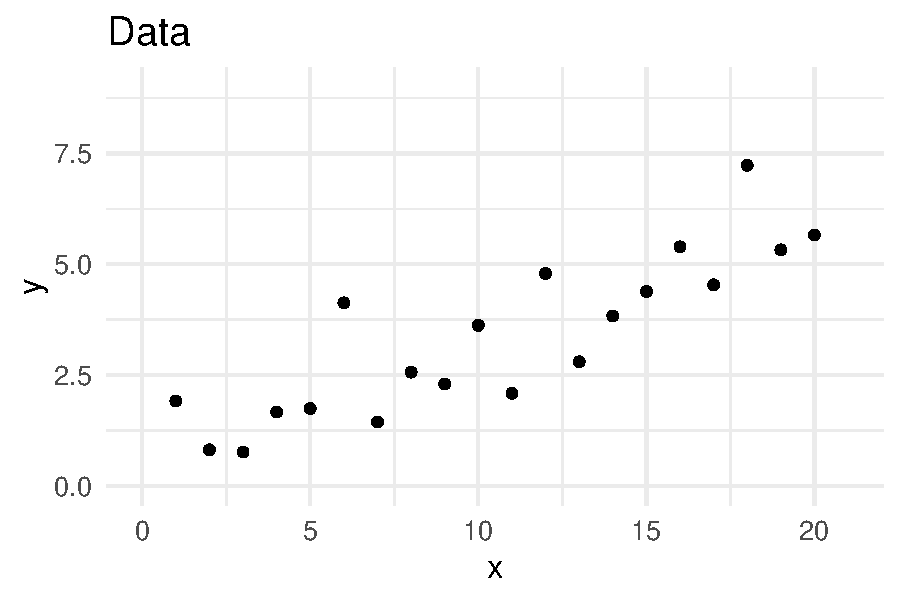
\includegraphics[width=8cm]{figs/fakel_data.pdf}}
  \only<2>{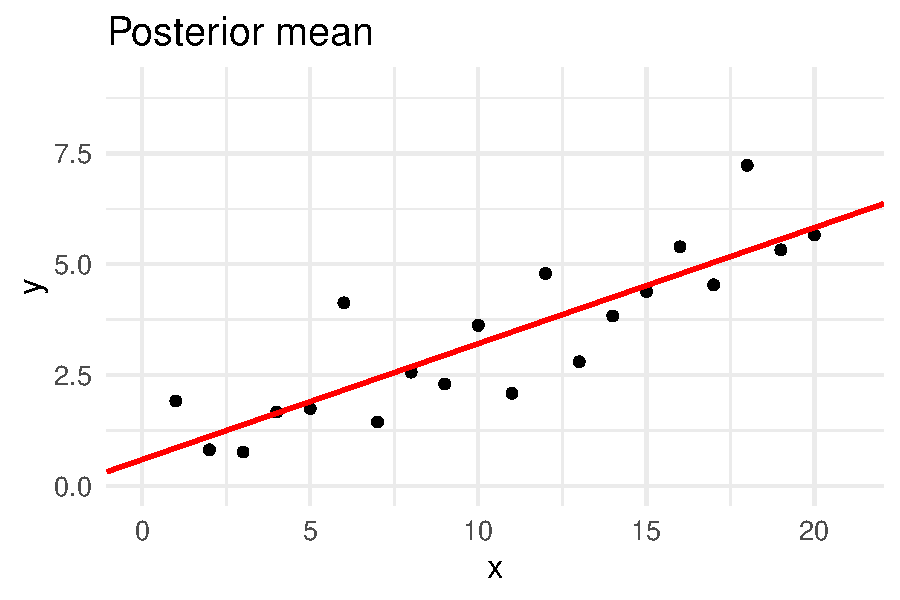
\includegraphics[width=8cm]{figs/fakel_postmean.pdf}}
  \only<3>{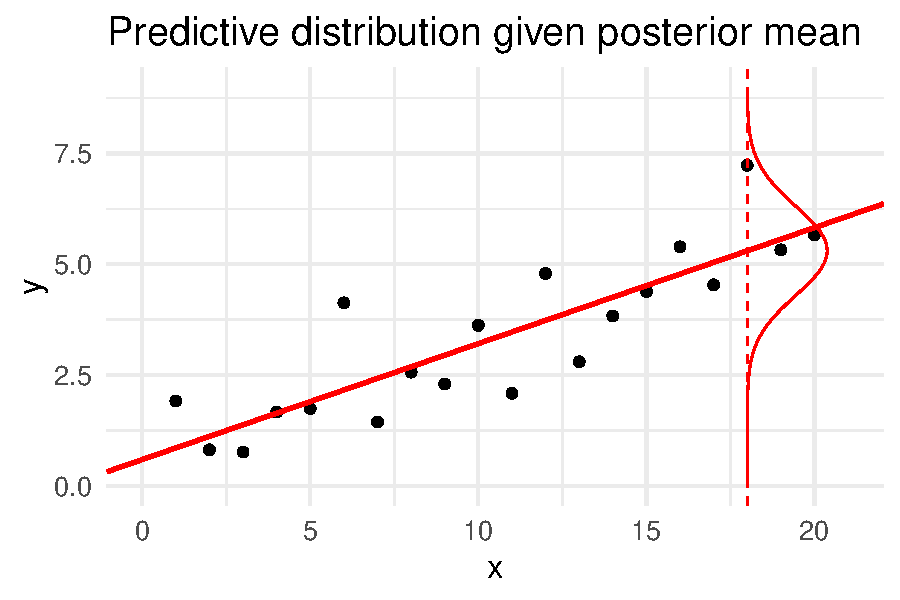
\includegraphics[width=8cm]{figs/fakel_postmeanpred.pdf}}
  \only<4>{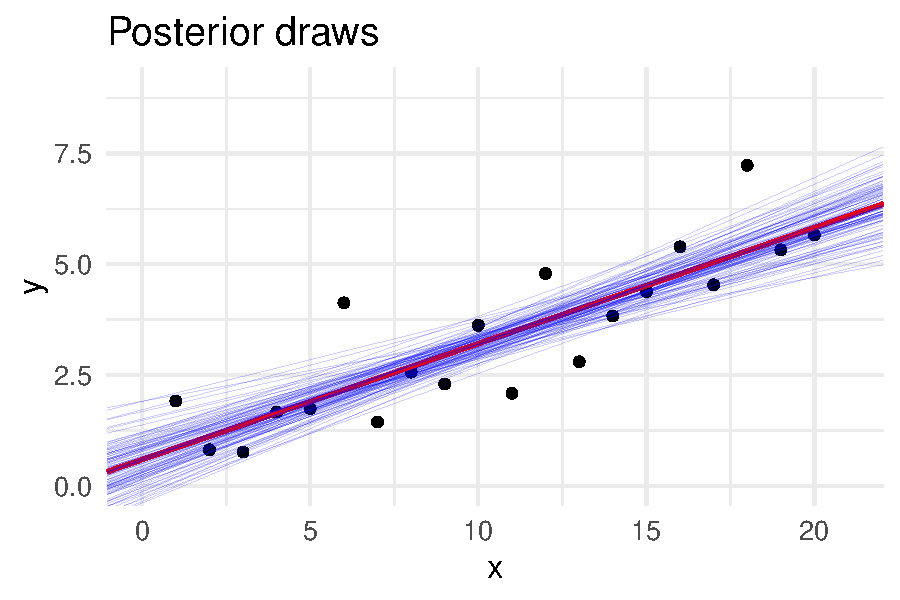
\includegraphics[width=8cm]{figs/fakel_postdraws.pdf}}
  \only<5>{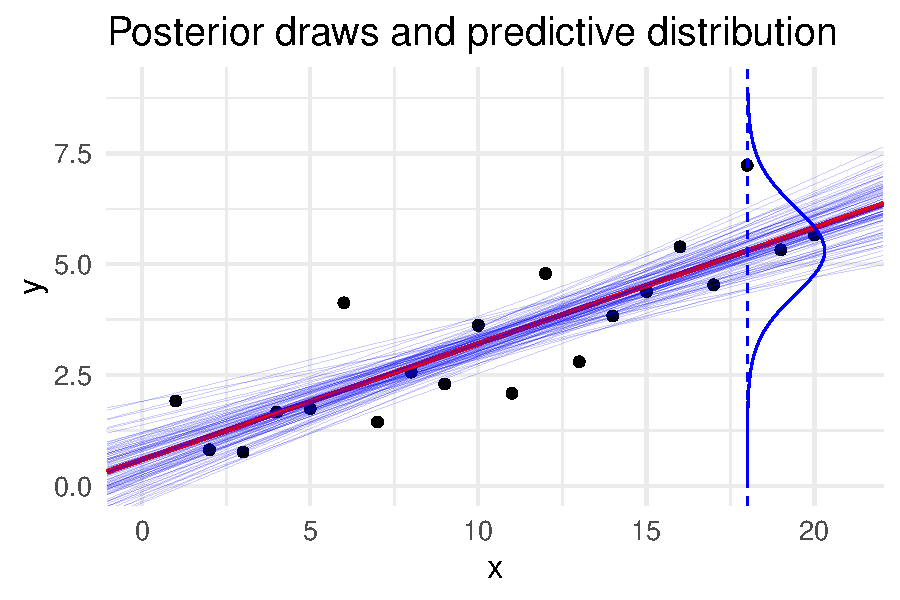
\includegraphics[width=8cm]{figs/fakel_postdrawspred.pdf}}
  \only<6>{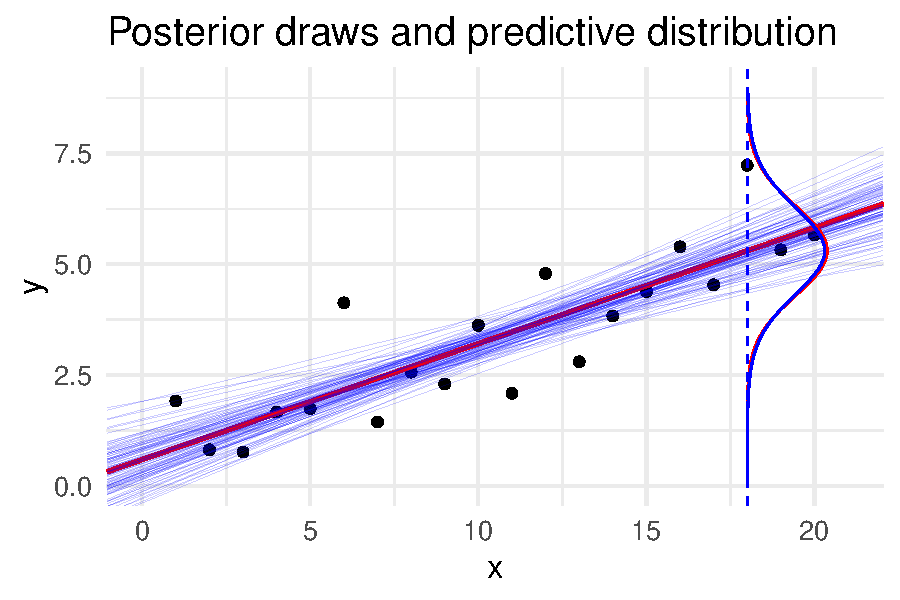
\includegraphics[width=8cm]{figs/fakel_postdrawspred2.pdf}}

\end{frame}
\begin{frame}

\frametitle{Monte Carlo and Posterior Draws}

  \begin{itemize}
  \item Assume we can get draws from $p(\theta \mid y)$
  \pause
  \item $\theta^{(s)}$ draws from $p(\theta \mid y)$ can be used
    \begin{itemize}
    \item<1-> for visualization
    \item<2-> to approximate expectations (integrals)
      \begin{align*}
        E_{p(\theta \mid y)}[\theta] = \int \theta p(\theta \mid y) \approx \frac{1}{S}\sum_{s=1}^{S} \theta^{(s)}
      \end{align*}
    \end{itemize}
    \item<3-> to approximate uncertainty intervals for $\theta$
  \end{itemize}

\end{frame}

\section{Multiple parameter models}
%\frame{\sectionpage}
\subsection{Marginalization}

\begin{frame}
\frametitle{Marginalization}

  \begin{itemize}
  \item Joint posterior distribution of multiple parameters
    \begin{align*}
      p(\theta_1,\theta_2 \mid y) \propto p(y \mid \theta_1,\theta_2)p(\theta_1,\theta_2)
    \end{align*}
  \pause
  \item {\color{uured} Marginalization}
      \begin{align*}
        p(\theta_1 \mid y) = \int p(\theta_1,\theta_2 \mid y) d\theta_2
      \end{align*}
      $p(\theta_1 \mid y)$ is a marginal distribution
       \vspace{0.5\baselineskip}
  \pause
 \item Goal is often to find marginal posterior of an interesting quantity
   \begin{itemize}
   \item a {\color{uured} parameter} $p(\theta|y)$
   \item a {\color{uured} potential observation} $p(\tilde{y}|y)$
   \end{itemize}
%    \item<2-> Monte Carlo approximation
%          \begin{align*}
%      p(\theta_1 \mid y) \approx  \frac{1}{S}\sum_{s=1}^{S} p(\theta_1,\theta_2^{(s)}\mid y),
%    \end{align*}
%    where $\theta_2^{(s)}$ are draws from $p(\theta_2 \mid y)$
  \end{itemize}

\end{frame}

\begin{frame}

\frametitle{Marginalization - predictive distribution}

  \begin{itemize}
\item Joint distribution of unknown future observation and parameters
   \begin{align*}
     p(\tilde{y},\theta \mid y) &= p(\tilde{y} \mid \theta,y) p(\theta \mid y)\\
      &= p(\tilde{y} \mid \theta) p(\theta \mid y) \qquad \text{(often)}
   \end{align*}
   \pause
  \item Marginalization over posterior distribution
      \begin{align*}
        p(\tilde{y} \mid y) & = \int p(\tilde{y} \mid \theta)p(\theta \mid y) d\theta\\
         & = \int p(\tilde{y}, \theta \mid y) d\theta
      \end{align*}
      $p(\tilde{y} \mid y)$ is a predictive distribution
  \end{itemize}

\end{frame}

\subsection{Gaussian}

\begin{frame}
\frametitle{Gaussian with unknown $\mu$ and $\sigma^2$}

\begin{itemize}
\item Observation model
  \begin{align*}
   \frac{1}{\sqrt{2\pi}\sigma}\exp\left(-\frac{1}{2\sigma^2}(y-\theta)^2 \right)
   \end{align*}
\item Uninformative prior
  \begin{align*}
    p(\mu,\sigma^2)\propto \sigma^{-2}
  \end{align*}
\end{itemize}

\end{frame}


\begin{frame}

\frametitle{Gaussian example}

  \only<1>{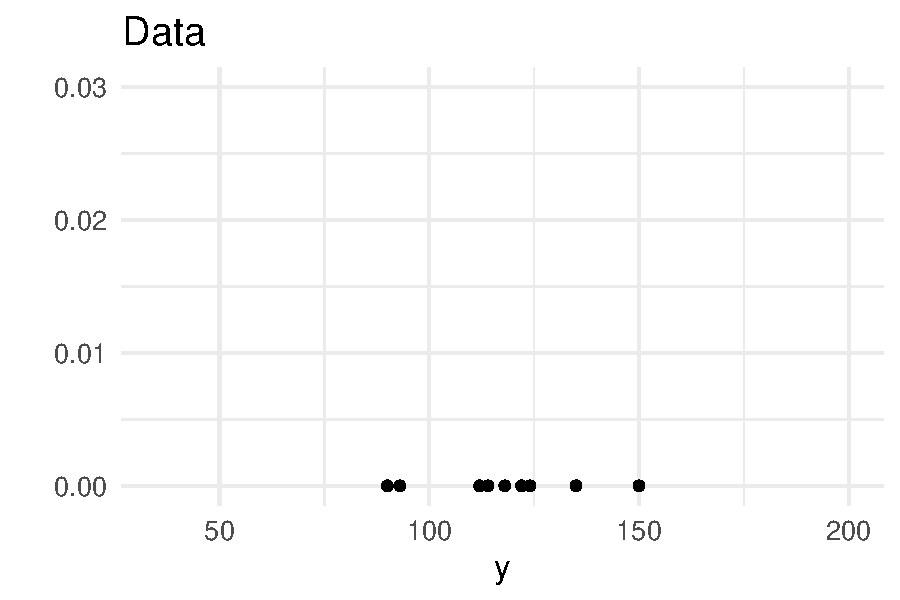
\includegraphics[width=8cm]{figs/fake3_data.pdf}}
  \only<2>{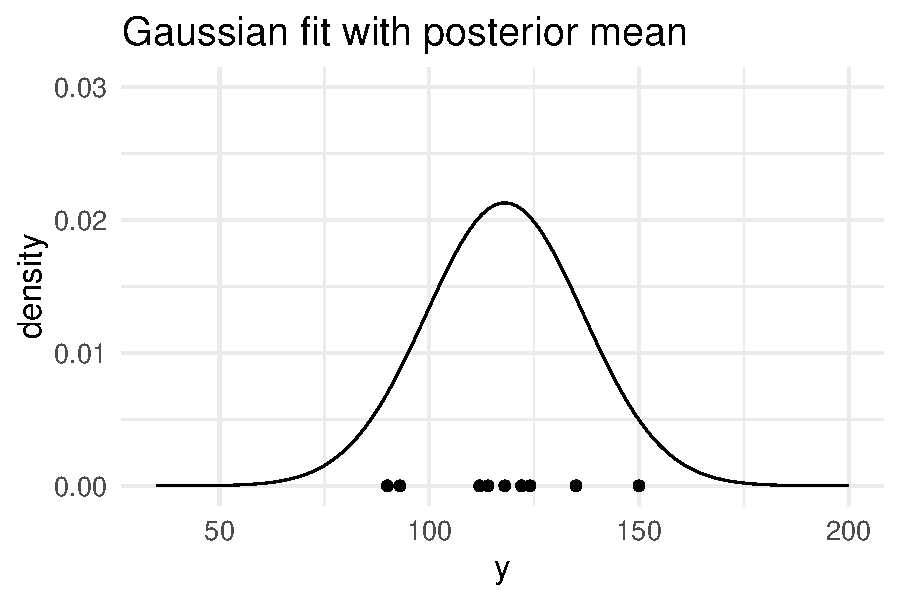
\includegraphics[width=8cm]{figs/fake3_postmean.pdf}}
  \only<3>{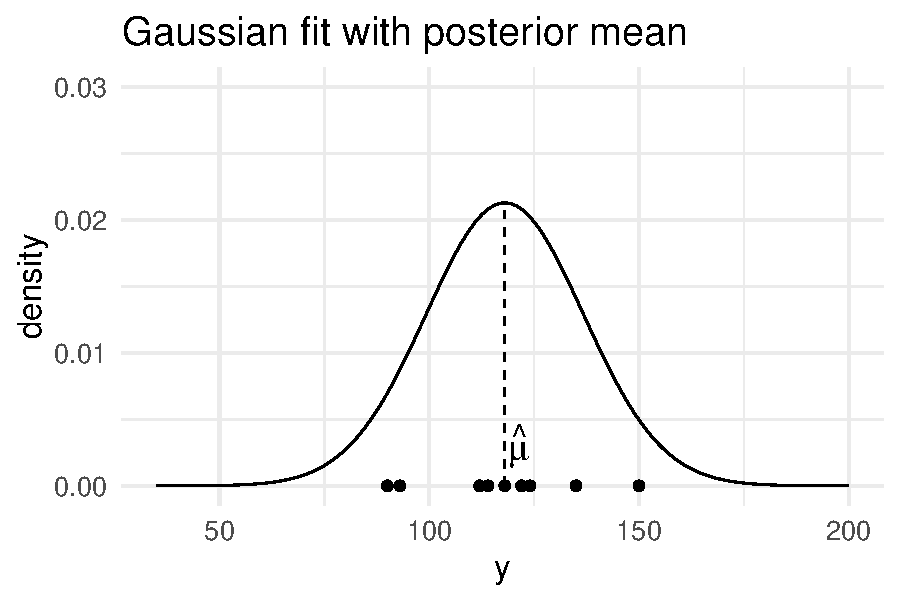
\includegraphics[width=8cm]{figs/fake3_postmeanmu.pdf}}
  \only<4>{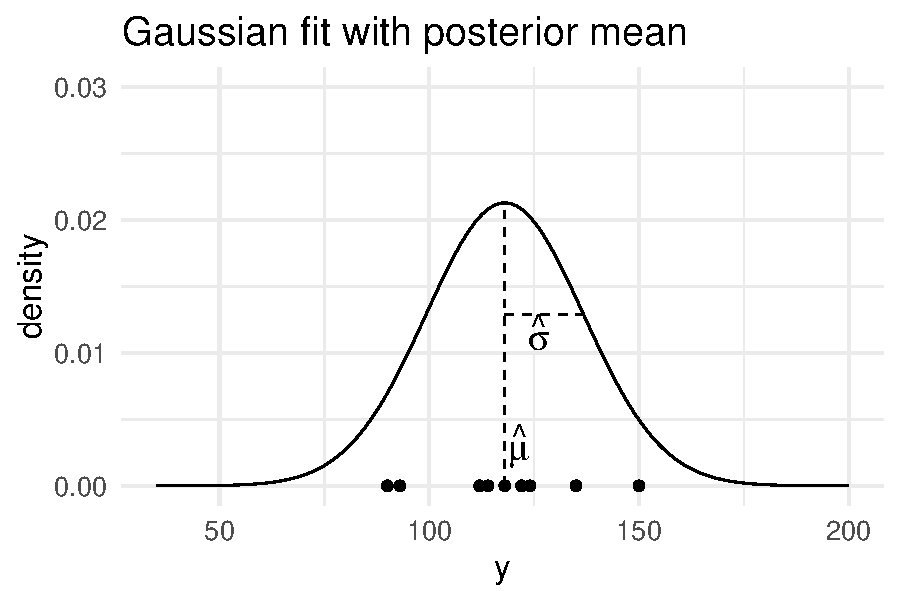
\includegraphics[width=8cm]{figs/fake3_postmeanmusigma.pdf}}
  \only<5>{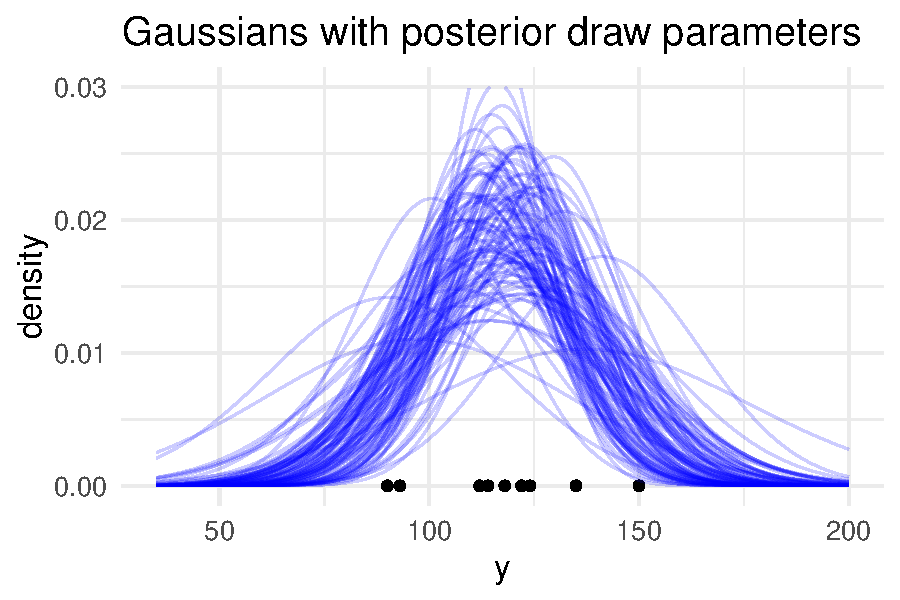
\includegraphics[width=8cm]{figs/fake3_postgaussiandraws.pdf}}
  \only<6>{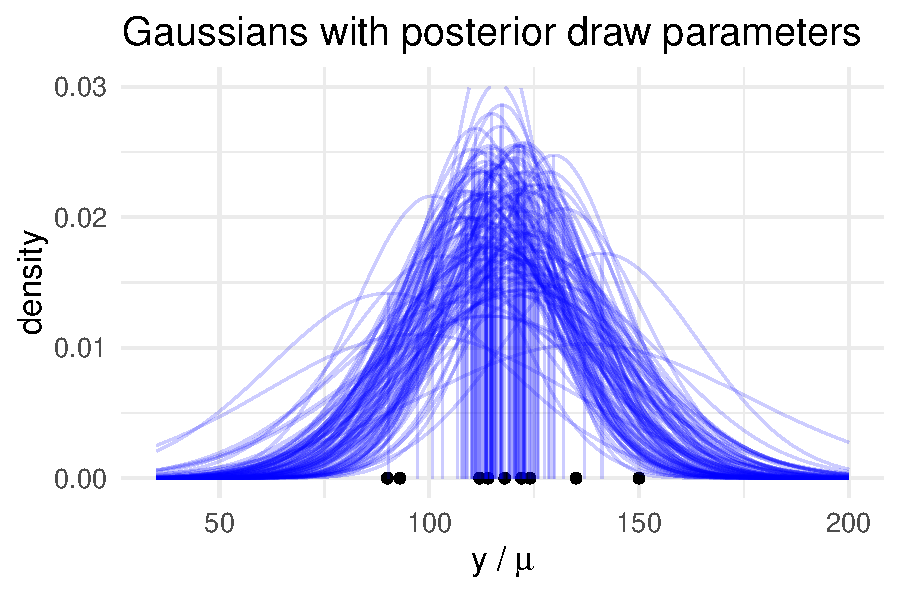
\includegraphics[width=8cm]{figs/fake3_postgaussianmudraws.pdf}}
  \only<7>{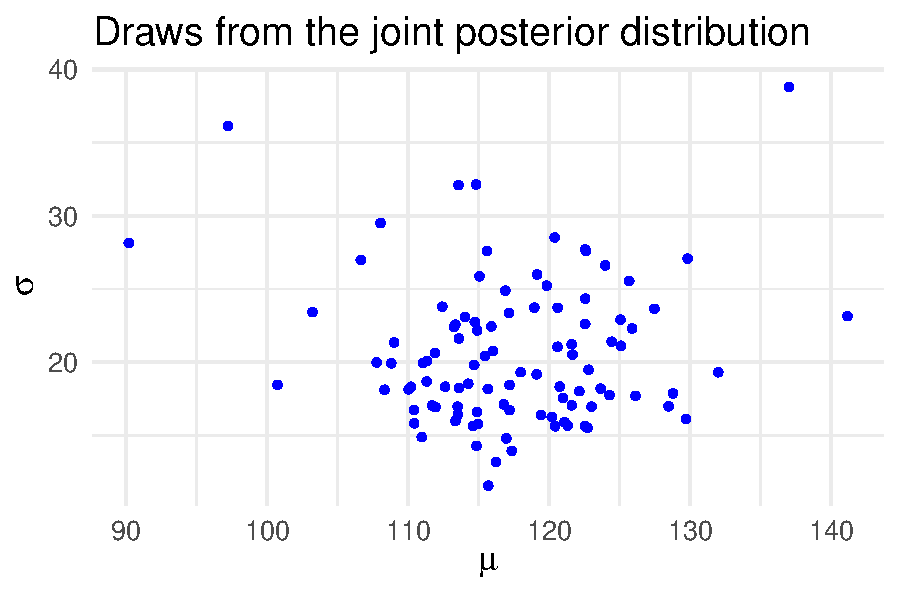
\includegraphics[width=8cm]{figs/fake3_postdraws100.pdf}}
  \only<8>{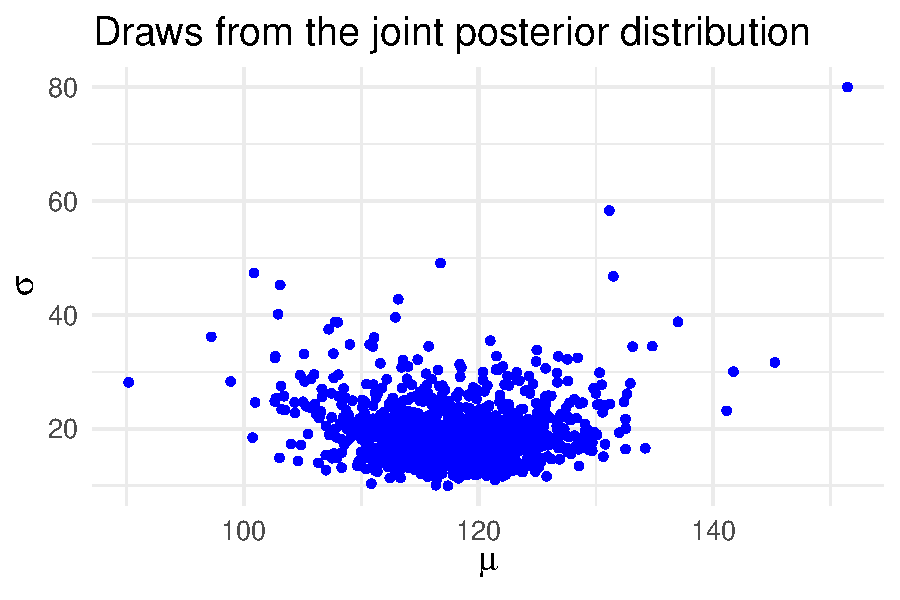
\includegraphics[width=8cm]{figs/fake3_postdraws.pdf}}
  \\
    \vspace{-\baselineskip}
  \only<2>{
    \begin{align*}
    p({\color{red} y} \mid  \mu, \sigma) = \frac{1}{\sqrt{2\pi}\sigma}\exp\left(-\frac{1}{2\sigma^2}({\color{red} y}-\mu)^2 \right)
    \end{align*}
  }
  \only<3>{
    \begin{align*}
    p(y \mid  {\color{red} \mu}, \sigma) = \frac{1}{\sqrt{2\pi}\sigma}\exp\left(-\frac{1}{2\sigma^2}(y-{\color{red} \mu})^2 \right)
    \end{align*}
  }
  \only<4>{
    \begin{align*}
    p(y \mid  \mu, {\color{red} \sigma}) = \frac{1}{\sqrt{2\pi}{\color{red} \sigma}}\exp\left(-\frac{1}{2{\color{red} \sigma}^2}(y-\mu)^2 \right)
    \end{align*}
  }
  \only<5->{
    \begin{align*}
      {\color{blue} \mu^{(s)}, \sigma^{(s)}} \sim p(\mu, \sigma  \mid  y)
    \end{align*}
    }

\end{frame}

\begin{frame}

  \vspace{-1\baselineskip}
  {\hfill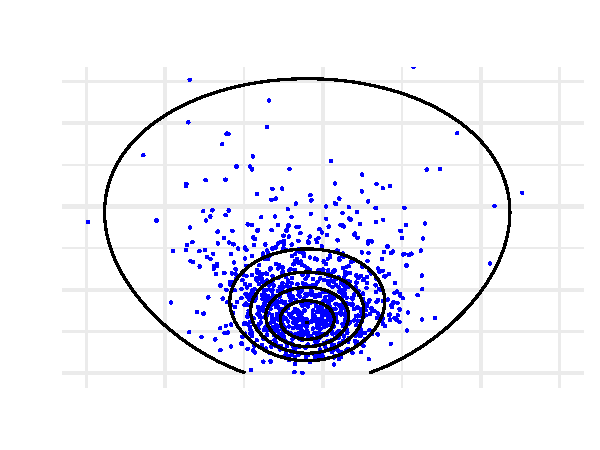
\includegraphics[width=5cm]{figs/fake3_joint1b.pdf}}\\
  \vspace{-5.5\baselineskip}
  Joint posterior\\
  \vspace{-.75\baselineskip}
  \begin{align*}
    {\color{blue} \mu^{(s)}, \sigma^{(s)}} & \sim p(\mu, \sigma  \mid  y) \\
    \uncover<2->{\text{with } p(\mu,\sigma^2) & \propto \sigma^{-2}} \\
    \only<3>{p(\mu,\sigma^2 \mid y) & \propto  \sigma^{-2}\prod_{i=1}^n\frac{1}{\sqrt{2\pi}\sigma}\exp\left(-\frac{1}{2\sigma^2}(y_i-\mu)^2\right)\\}
    \uncover<4->{p(\mu,\sigma^2 \mid y) & \propto  \sigma^{-n-2}\exp\left(-\frac{1}{2\sigma^2}\sum_{i=1}^n(y_i-\mu)^2\right)}\\
    \uncover<5->{&  = \sigma^{-n-2}\exp\left(-\frac{1}{2\sigma^2}\left[\sum_{i=1}^n(y_i-\bar{y})^2+n(\bar{y}-\mu)^2\right]\right)}\\
    \uncover<5->{\color{gray} \text{where } \bar{y} & \color{gray} = \frac{1}{n}\sum_{i=1}^n y_i }\\
    \uncover<6->{&  = \sigma^{-n-2}\exp\left(-\frac{1}{2\sigma^2}\left[(n-1)s^2+n(\bar{y}-\mu)^2\right]\right)}\\
    \uncover<6->{\color{gray} \text{where }  s^2 & \color{gray} =\frac{1}{n-1}\sum_{i=1}^n(y_i-\bar{y})^2}
  \end{align*}

\end{frame}

\begin{frame}{Gaussian: Completing the square}

  \vspace{-\baselineskip}
 \begin{align*}
   &\onslide<1->{\sum_{i=1}^n(y_i-\mu)^2}\\
   &\onslide<2->{\sum_{i=1}^n(y_i^2-2 y_i \mu + \mu^2)}\\
\pause
   &\onslide<3->{\sum_{i=1}^n(y_i^2-2 y_i \mu + \mu^2 -\bar{y}^2 + \bar{y}^2 - 2 y_i \bar{y} + 2 y_i \bar{y})}\\
   &\onslide<4->{\sum_{i=1}^n(y_i^2-2 y_i \bar{y} + \bar{y}^2) + \sum_{i=1}^n(\mu^2 - 2 y_i \mu -\bar{y}^2  + 2 y_i \bar{y})}\\
   &\onslide<5->{\sum_{i=1}^n(y_i-\bar{y})^2 + n(\mu^2 -  2\bar{y}\mu -\bar{y}^2  + 2 \bar{y}\bar{y})}\\
   &\onslide<6->{\sum_{i=1}^n(y_i-\bar{y})^2 + n(\bar{y}-\mu)^2}
 \end{align*}

\end{frame}

\begin{frame}{Marginal $p(\mu)$ and $p(\sigma^2)$}

  {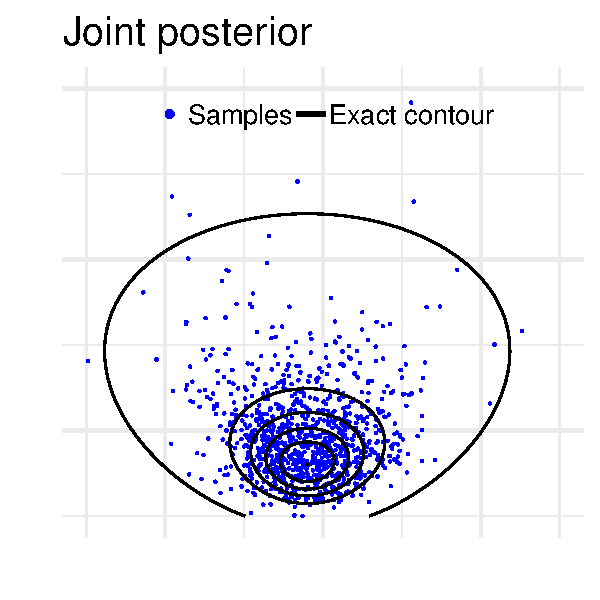
\includegraphics[width=4cm]{figs/fake3_joint1.pdf}}
  \uncover<2->{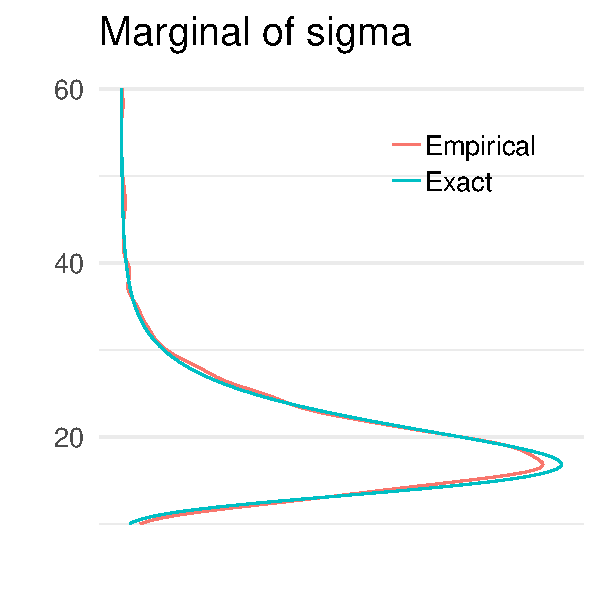
\includegraphics[width=4cm]{figs/fake3_marginalsigma.pdf}}\\
  \uncover<1->{\vspace{-\baselineskip}
    \begin{minipage}{4cm}
      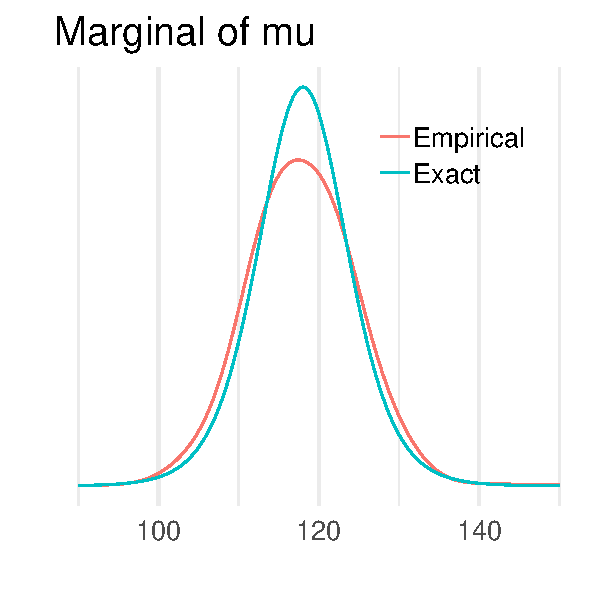
\includegraphics[width=4cm]{figs/fake3_marginalmu.pdf}
    \end{minipage}
  }
  \begin{minipage}{4cm}
    \vspace{-2\baselineskip}
     \begin{align*}
       {\color{blue} \mu^{(s)}, \sigma^{(s)}} & \sim p(\mu, \sigma  \mid  y) \\
       \uncover<2->{\text{marginals}\\
       p(\mu \mid y) & = \int p(\mu,\sigma \mid y) d \sigma }\\
       \uncover<2->{p(\sigma \mid y) & = \int p(\mu,\sigma \mid y) d \mu }
     \end{align*}
  \end{minipage}

\end{frame}

\begin{frame}{Marginal $p(\mu|y)$ and $p(\sigma^2|y)$}

   {Marginal posterior $p(\sigma^2 \mid y)$ (easier for $\sigma^2$ than $\sigma$)}
    \begin{eqnarray*}
    p(\sigma^2 \mid y) & \propto & \int
    p(\mu,\sigma^2 \mid y) d\mu\\
    \uncover<2->{& \propto & \int
    \sigma^{-n-2}\exp\left(-\frac{1}{2\sigma^2}\left[(n-1)s^2+n(\bar{y}-\mu)^2\right]\right) d\mu\\}
    & \uncover<3->{\propto &
    \sigma^{-n-2}\exp\left(-\frac{1}{2\sigma^2}(n-1)s^2\right) \cdot} \\
    & \uncover<3->{&\int
    \exp\left(-\frac{n}{2\sigma^2}(\bar{y}-\mu)^2\right) d\mu}\\
    \uncover<4->{\color{gray} Note! & & \color{gray} \int \frac{1}{\sqrt{2\pi}\sigma} \exp\left(-\frac{1}{2\sigma^2}(y-\theta)^2\right) d\theta = 1}\\
    & \uncover<5->{\propto &
    \sigma^{-n-2}\exp\left(-\frac{1}{2\sigma^2}(n-1)s^2\right)\sqrt{2\pi\sigma^2/n}}\\
    & \uncover<6->{\propto &
    (\sigma^2)^{-(n+1)/2}\exp\left(-\frac{(n-1)s^2}{2\sigma^2}\right)} \\
    \uncover<7->{p(\sigma^2 \mid y) &  = &  \Invchi2(\sigma^2 \mid n-1,s^2)}
  \end{eqnarray*}

\end{frame}

\begin{frame}{Gaussian - non-informative prior}

  \begin{itemize}
  \item[] Known mean
    \begin{align*}
      \sigma^2 \mid y & \sim \Invchi2(n,v)\\
      \text{where} \quad v&=\frac{1}{n}\sum_{i=1}^{n}(y_i-\theta)^2
    \end{align*}
    \pause
  \item[] Unknown mean
    \begin{align*}
      \sigma^2 \mid y & \sim \Invchi2(n-1,s^2)\\
      \text{where} \quad s^2&=\frac{1}{n-1}\sum_{i=1}^{n}(y_i-\bar{y})^2
  \end{align*}
    \end{itemize}

\end{frame}

\begin{frame}
  \frametitle{Gaussian - non-informative prior}

 \begin{itemize}
  \item Marginal posterior $p(\mu \mid y)$
   \begin{equation*}
     p(\mu \mid y)=\int_0^\infty p(\mu \mid \sigma^2,y)p(\sigma^2 \mid y)d\sigma^2
    \end{equation*}
   \item Marginal posterior of $\mu$, a mixture of normal
     distributions where mixing density is the marginal posterior of
      $\sigma^2$
\end{itemize}

\end{frame}

\begin{frame}

  {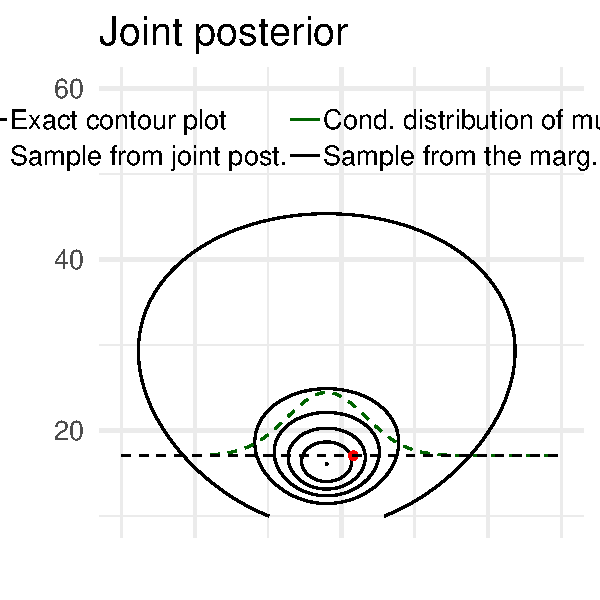
\includegraphics[width=4cm]{figs/fake3_joint2.pdf}}
  {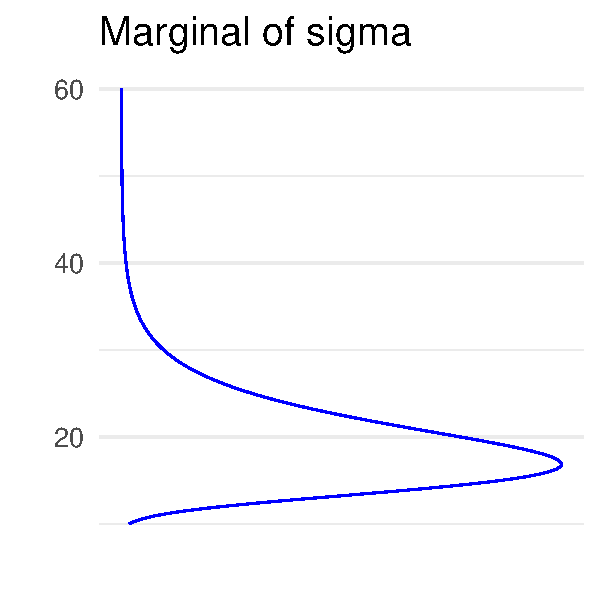
\includegraphics[width=4cm]{figs/fake3_marginalsigma2.pdf}}\\\vspace{-\baselineskip}
  \begin{minipage}[b][4cm][t]{4cm}
  \only<1-3>{~}
  \only<4>{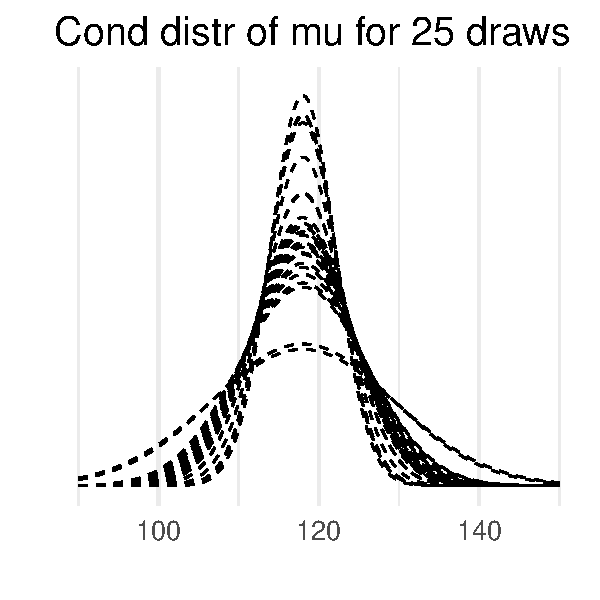
\includegraphics[width=4cm]{figs/fake3_condsmu.pdf}}
  \only<5>{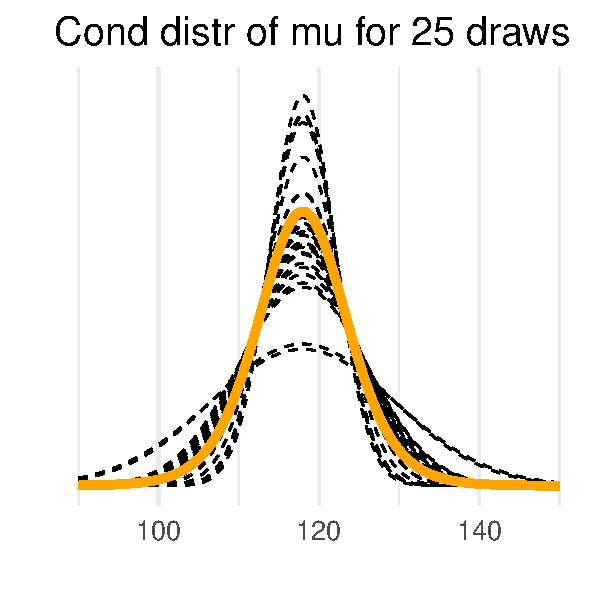
\includegraphics[width=4cm]{figs/fake3_condsmumean.pdf}}
  \only<6>{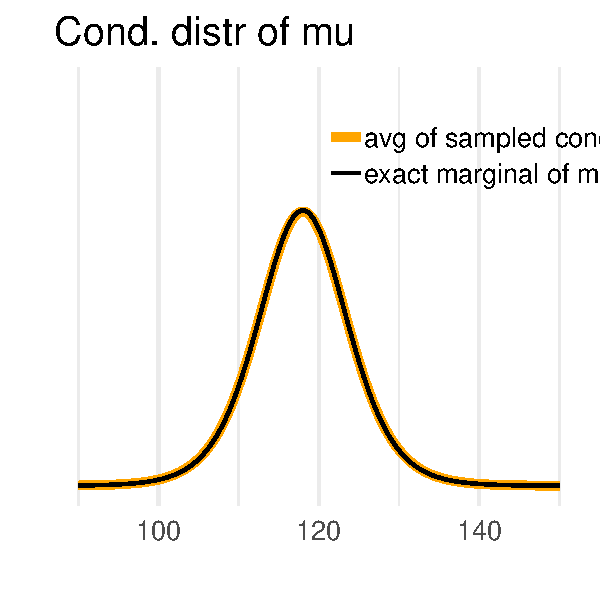
\includegraphics[width=4cm]{figs/fake3_marginalmu2.pdf}}
  \end{minipage}
  \makebox[5cm][t]{
  \begin{minipage}[b][4cm][t]{4cm}
    \small
    \vspace{.25\baselineskip}
    Factorization
    %\vspace{-5\baselineskip}
     \begin{align*}
       p(\mu,\sigma^2 \mid y) & = {\color{uured} p(\mu \mid \sigma^2,y)}{\color{blue} p(\sigma^2 \mid y)} \\
       \uncover<2->{(\sigma^2)^{(s)} & \sim {\color{blue} p(\sigma^2 \mid y)}} \\
       \uncover<3->{\color{uured} p(\mu \mid  (\sigma^2)^{(s)},y) & = \N(\mu \mid \bar{y},(\sigma^2)^{(s)}/n)}\\
       \uncover<5->{p(\mu \mid y) & \approx {\color{orange} \frac{1}{S}\sum_{s=1}^S \N(\mu \mid \bar{y},(\sigma^2)^{(s)}/n)}}
     \end{align*}
  \end{minipage}
}
\end{frame}

\begin{frame}[fragile]{Marginal posterior $p(\mu \mid y)$}

    \begin{align*}
      p(\mu \mid y)&=\int_0^\infty p(\mu,\sigma^2 \mid y)d\sigma^2\\
      \uncover<2->{ & \propto \int_0^\infty \sigma^{-n-2}\exp\left(-\frac{1}{2\sigma^2}\left[{\only<3>{\color{blue}}(n-1)s^2+n(\bar{y}-\mu)^2}\right]\right) d\sigma^2}
    \end{align*}
   \uncover<3->{Transformation (integration by substitution)\\}
    \vspace{-1\baselineskip}
    \begin{align*}
      \uncover<3->{A=\only<3>{\color{blue}}(n-1)s^2+n(\mu-\bar{y})^2}\uncover<4->{\quad \text{and} \quad {\only<4-5>{\color{blue}}z=\frac{A}{2\sigma^2}}}
    \end{align*}
    \begin{align*}
      \uncover<4->{d{\only<4-5>{\color{blue}}z} = \left( -\frac{A}{2 (\sigma^2)^2}\right) d\sigma^2}
    \end{align*}
%  \vspace{-\baselineskip}
    \begin{align*}
     \uncover<5->{p(\mu \mid y)&\propto {\only<7>{\color{blue}}A^{-n/2}}\int_0^\infty {\only<5>{\color{blue}}z}^{(n-2)/2}\exp(-{\only<5>{\color{blue}}z})d{\only<5>{\color{blue}}z}}
   \uncover<6->{\intertext{\color{gray} Recognize gamma integral\, $\Gamma(u) = \int_0^\infty x^{u-1}\exp(-x)dx$}}
    \uncover<7->{&\propto {\only<7>{\color{blue}}[(n-1)s^2+n(\mu-\bar{y})^2]^{-n/2}}\\}
    \end{align*}

\end{frame}


\begin{frame}[fragile]{Marginal posterior $p(\mu \mid y)$}

    \begin{align*}
    \uncover<1->{p(\mu|y) &\propto {\only<1>{\color{blue}}[(n-1)s^2+n(\mu-\bar{y})^2]^{-n/2}}\\}
    \uncover<2->{&\propto \left[1+\frac{n(\mu-\bar{y})^2}{(n-1)s^2}\right]^{-n/2}\\}
    \uncover<3->{p(\mu \mid y) & = t_{n-1}(\mu \mid \bar{y},s^2/n) \color{gray} \quad \text{Student's $t$}}
    \end{align*}

\end{frame}



\begin{frame}

  {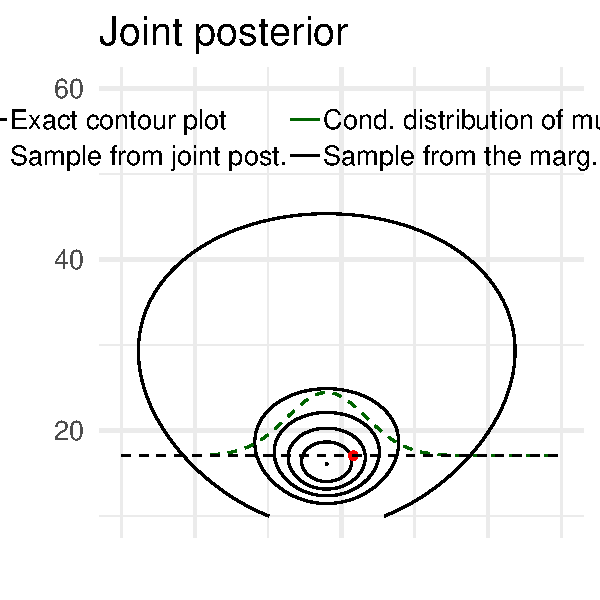
\includegraphics[width=4cm]{figs/fake3_joint2.pdf}}
  {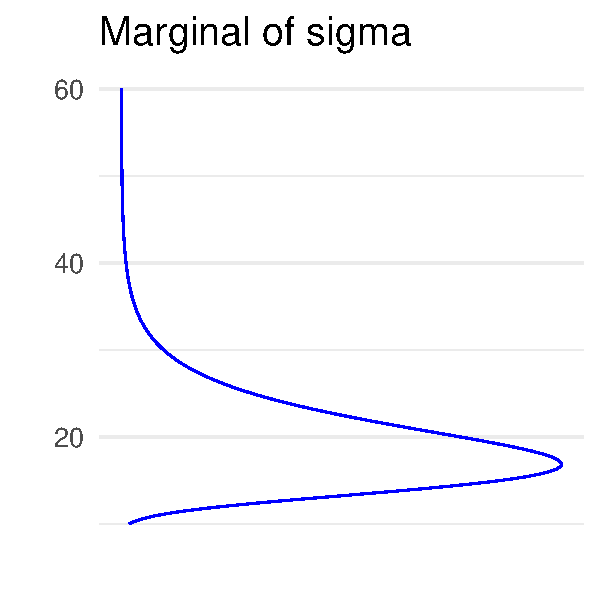
\includegraphics[width=4cm]{figs/fake3_marginalsigma2.pdf}}\\\vspace{-\baselineskip}
  % \begin{minipage}[b][5cm][t]{5cm}
  % {~}
  % \end{minipage}
  \makebox[4cm][t]{
    \hspace{-.7cm}
    \begin{minipage}[b][5cm][t]{5cm}
      \vspace{0.75\baselineskip}

    { \small Predictive distribution for new $\tilde{y}$}
    %\vspace{-2.75\baselineskip}
    \begin{align*}
      \only<6> {\color{orange}} \scriptstyle p(\tilde{y} \mid y) & \scriptstyle = \int p(\tilde{y} \mid \mu,\sigma)p(\mu,\sigma \mid y)d\mu\sigma\\
      \uncover<2->{{\color{red} \scriptstyle \mu^{(s)}, \sigma^{(s)}} & \scriptstyle \sim p(\mu, \sigma  \mid  y)}\\
      \uncover<3->{{\color{red} \scriptstyle \tilde{y}^{(s)}} & \scriptstyle \sim \color{blue} p(\tilde{y} \mid \mu^{(s)},\sigma^{(s)})}
     \end{align*}
   \end{minipage}
   }
  \begin{minipage}[b][5cm][t]{5cm}
  \only<1-2>{~}
  \only<3>{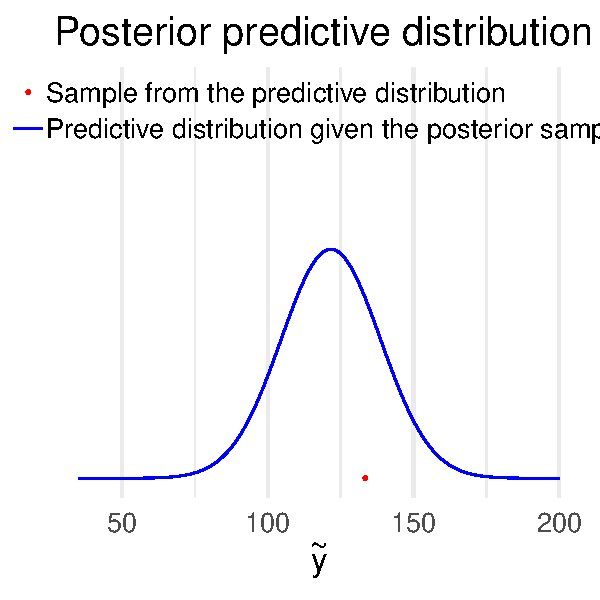
\includegraphics[width=4cm]{figs/fake3_pred1.pdf}}
  \only<4>{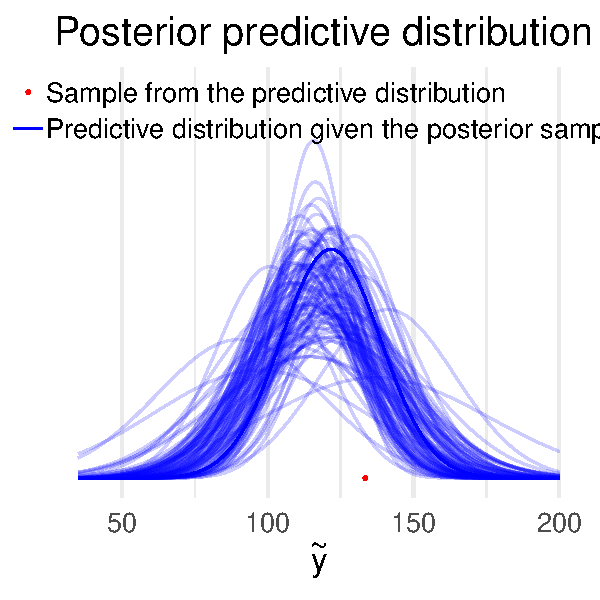
\includegraphics[width=4cm]{figs/fake3_pred1s.pdf}}
  \only<5>{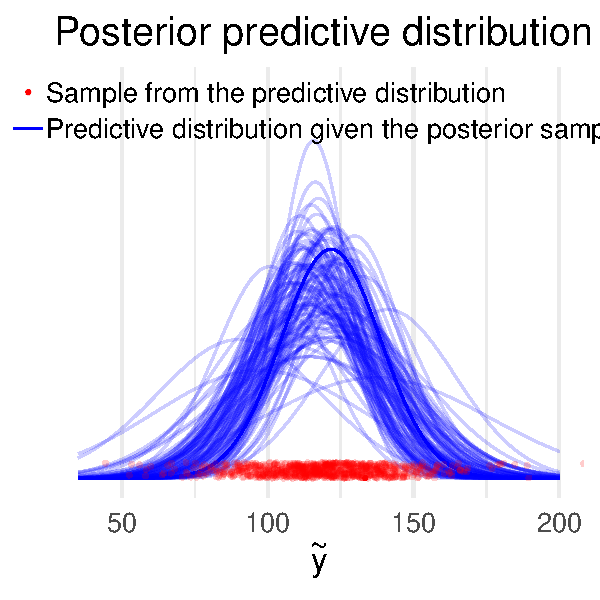
\includegraphics[width=4cm]{figs/fake3_pred1ss.pdf}}
  \only<6>{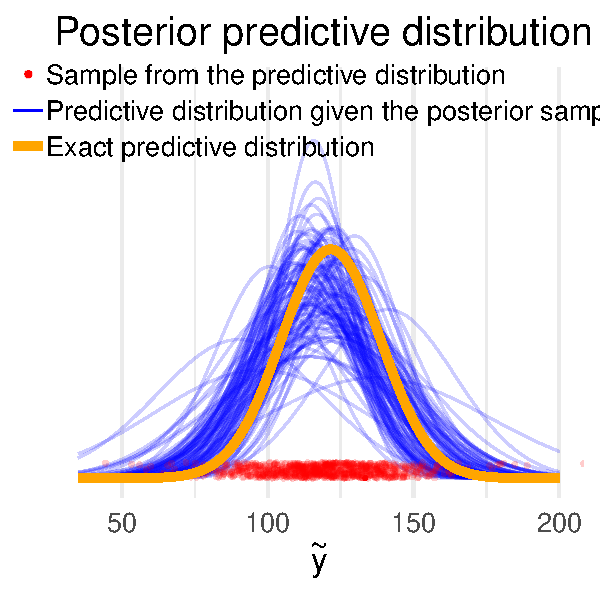
\includegraphics[width=4cm]{figs/fake3_pred1ss_exact.pdf}}
  \end{minipage}
\end{frame}


\begin{frame}{Gaussian - posterior predictive distribution}

   Posterior predictive distribution given known variance
    \begin{align*}
      p(\tilde{y} \mid \sigma^2,y) & = \int p(\tilde{y} \mid \mu,\sigma^2)p(\mu \mid \sigma^2,y)d\mu\\
       \uncover<2->{& = \int \N(\tilde{y} \mid \mu,\sigma^2)\N(\mu \mid \bar{y},\sigma^2/n)d\mu\\ }
       \uncover<3->{& = \N(\tilde{y} \mid \bar{y},(1+{\textstyle \frac{1}{n}})\sigma^2)}
    \uncover<4->{\intertext{\, \, \, this is up to scaling factor same as $p(\mu \mid \sigma^2,y)$}}
      \uncover<5->{p(\tilde{y} \mid y) & = t_{n-1}(\tilde{y} \mid \bar{y},(1+{\textstyle \frac{1}{n}})s^2)}
    \end{align*}

\end{frame}

\subsection{Example}

\begin{frame}{Simon Newcomb's light of speed experiment in 1882}

  {\small
  Newcomb measured ($n=66$) the time required for light to travel from
  his laboratory on the Potomac River to a mirror at the base of the
  Washington Monument and back, a total distance of 7422 meters.}
  \begin{center}
    \vspace{-0.5\baselineskip}
    {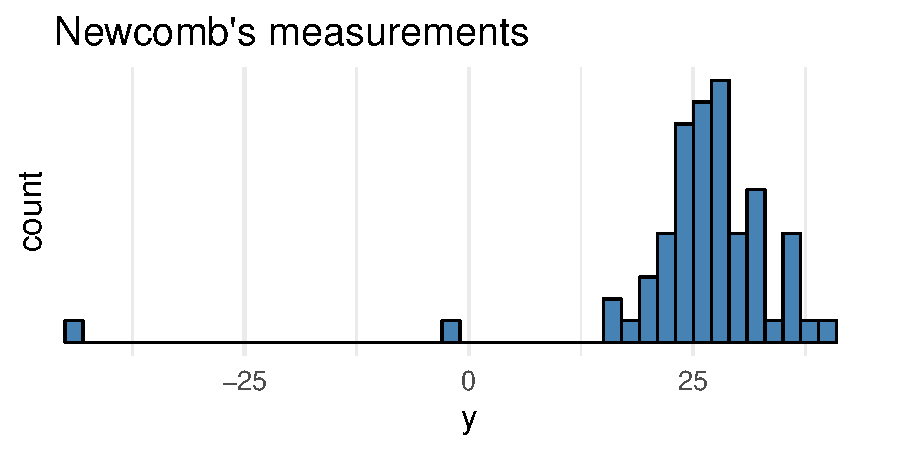
\includegraphics[width=6cm]{figs/newcomb_data.pdf}}\\
    \vspace{-1\baselineskip}
    \only<1>{\phantom{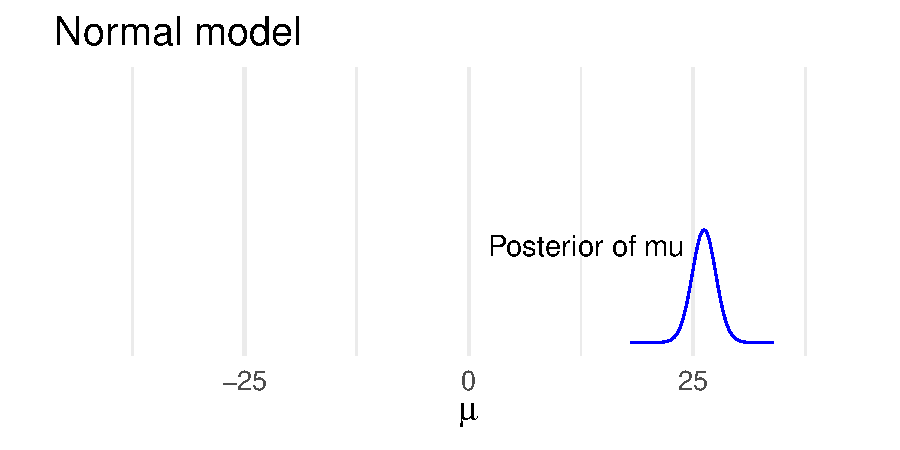
\includegraphics[width=6cm]{figs/newcomb_posterior1.pdf}}}
    \only<2>{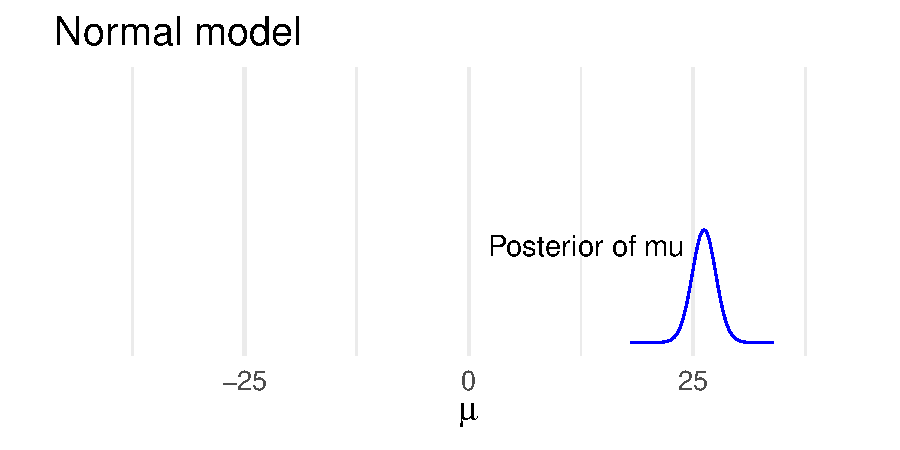
\includegraphics[width=6cm]{figs/newcomb_posterior1.pdf}}
    \only<3>{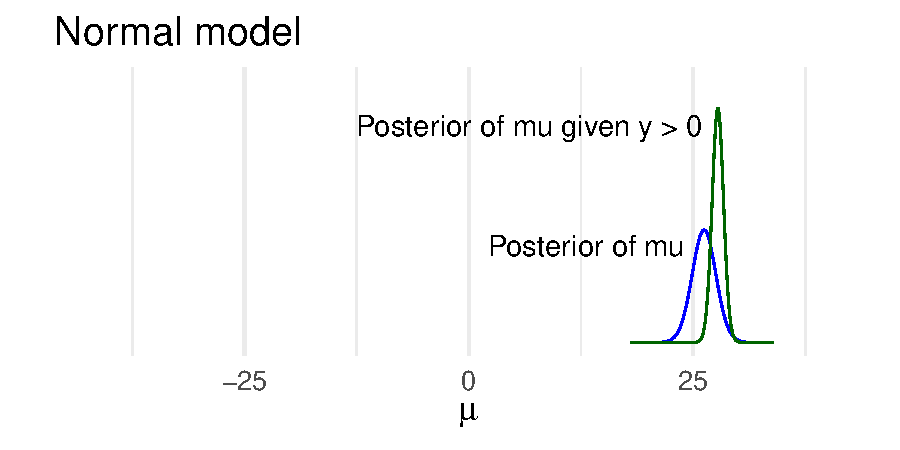
\includegraphics[width=6cm]{figs/newcomb_posterior2.pdf}}
    \only<4>{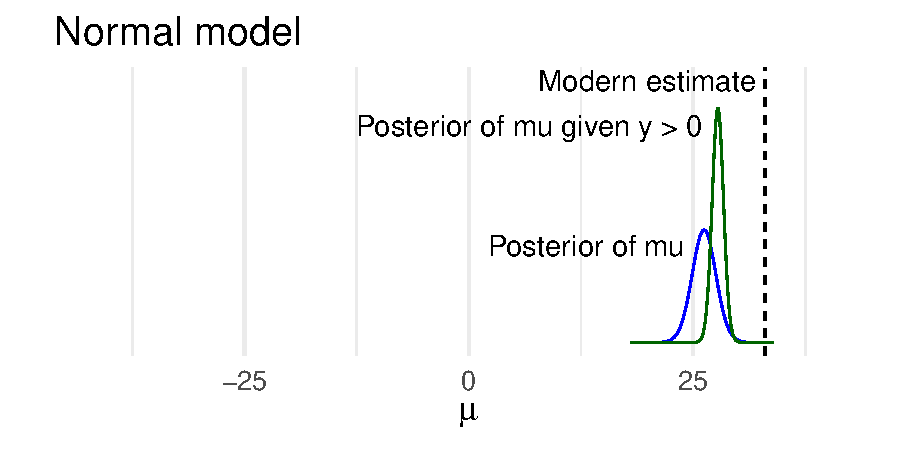
\includegraphics[width=6cm]{figs/newcomb_posterior3.pdf}}
  \end{center}

\end{frame}

\subsection{Gaussian - conjugate prior}

\begin{frame}{Gaussian - conjugate prior}

  \begin{itemize}
  \item[-] Conjugate prior has to have a form
    $p(\sigma^2)p(\mu \mid \sigma^2)$\\
    \pause
  \item[-] Handy parameterization
    \begin{align*}
      \mu \mid \sigma^2 & \sim \mathrm{N}(\mu_0,\sigma^2/\kappa_0)\\
      \sigma^2 & \sim \Invchi2(\nu_0,\sigma_0^2)
    \end{align*}
    which can be written as
    \begin{align*}
      p(\mu,\sigma^2)=\NInvchi2(\mu_0,\sigma_0^2/\kappa_0;\nu_0,\sigma_0^2)
    \end{align*}
    \pause
  \item[-] $\mu$ and $\sigma^2$ are a priori dependent
    \begin{itemize}
      \item[-] if $\sigma^2$ is large, then $\mu$ has wide prior
    \end{itemize}
  \end{itemize}

\end{frame}

\begin{frame}{Gaussian - conjugate prior}

  Joint posterior (exercise 3.9)
    \begin{align*}
      p(\mu,\sigma^2 \mid y)=\NInvchi2(\mu_n,\sigma_n^2/\kappa_n;\nu_n,\sigma_n^2)
    \end{align*}
    where
    \begin{align*}
      \mu_n & = \frac{\kappa_0}{\kappa_0+n}\mu_0 + \frac{n}{\kappa_0+n}\bar{y} \\
      \kappa_n & = \kappa_0+n \\
      \nu_n & = \nu_0+n \\
      \nu_n\sigma_n^2 & =\nu_0\sigma_0^2 + (n-1)s^2 +
      \frac{\kappa_0 n}{\kappa_0+n}(\bar{y}-\mu_0)^2
    \end{align*}

\end{frame}

\begin{frame}
 \frametitle{Gaussian - conjugate prior}

  \begin{itemize}
 \item Conditional $p(\mu \mid \sigma^2,y)$
    \begin{align*}
     \mu \mid \sigma^2,y & \sim \mathrm{N}(\mu_n,\sigma^2/\kappa_n)\\
     & =  \mathrm{N}\left(\frac{\frac{\kappa_0}{\sigma^2}\mu_0+\frac{n}{\sigma^2}\bar{y}}{\frac{\kappa_0}{\sigma^2}+\frac{n}{\sigma^2}},\frac{1}{\frac{\kappa_0}{\sigma^2}+\frac{n}{\sigma^2}}\right)
    \end{align*}
  \vspace{-2mm}
  \pause
 \item Marginal $p(\sigma^2 \mid y)$
  \begin{align*}
      \sigma^2 \mid y \sim \Invchi2(\nu_n,\sigma_n^2)
   \end{align*}
    \vspace{-6mm}
  \pause
  \item Marginal $p(\mu \mid y)$
   \begin{align*}
     \mu \mid y \sim t_{\nu_n}(\mu \mid \mu_n,\sigma_n^2/\kappa_n)
   \end{align*}
  \end{itemize}

\end{frame}


\subsection{Multinomial model}

\begin{frame}{Multinomial model for categorical data}

  \begin{itemize}
  \item[-] Extension of binomial to $K$ categories
  \item[-] Observation model (Categorical distribution, $n=1$)\\
  $y_i = (0,1,0,0,0)$ - {\color{uured} what is $K$ here?}
  \pause
    \begin{align*}
      p(y  \mid  \theta) \propto \prod_{k=1}^K \theta_j^{y_j},
    \end{align*}
    \begin{align*}
      \text{where } \sum_k^K \theta_k = 1\,, \text{ and } \forall \theta_k > 0
    \end{align*}
  \item[-] {\color{uured} What is important when choosing the prior for $\theta$?}
  \pause
  \item[-] Conjugate prior: The Dirichlet distribution
  \begin{align*}
    p(\theta) \propto \prod_{k=1}^K \theta_k^{\alpha_k-1},
  \end{align*}
  \begin{align*}
      \text{where } \forall \alpha_k > 0
  \end{align*}
  \end{itemize}
\end{frame}

\begin{frame}{Multinomial model for categorical data: The posterior}

  \begin{itemize}
  \item The posterior $p(\theta|y)$
    \begin{align*}
      p(\theta \mid y) & \propto p(y \mid \theta) p(\theta)\\
       \uncover<2->{& \propto \prod_{k=1}^K \theta_k^{\alpha_k-1} \prod^n_i \prod_{k=1}^K \theta_k^{y_{k,i}}}\\
       \uncover<3->{& = \prod_{k=1}^K \theta_k^{\alpha_k-1} \prod_{k=1}^K \theta_k^{\sum^n_i y_{k,i}}}\\
       \uncover<4->{& = \prod_{k=1}^K \theta_k^{\alpha_k - 1 + \sum^n_i y_{k,i}}}
    \end{align*}

  \uncover<5->{\item The posterior is $p(\theta|y) = \text{Dir}(\alpha + \sum y)$}
  \end{itemize}
\end{frame}

\subsection{Multivariate Gaussian}

\begin{frame}{Multivariate Gaussian}

  \begin{itemize}
  \item[-] Observation model
    \begin{align*}
      p(y \mid \mu,\Sigma)\propto  \mid \Sigma \mid ^{-1/2}
      \exp\left( -\frac{1}{2} (y-\mu)^T \Sigma^{-1} (y-\mu)\right),
    \end{align*}
    \begin{align*}
      \text{where } y \in \mathcal{R}^D\,
    \end{align*}
  \item[-] See BDA3 p. 72--
  \item[-] New recommended LKJ-prior mentioned in Appendix A, see more
    in Stan manual
  \end{itemize}
\end{frame}

\section{Bioassay example}

\begin{frame}{Bioassay}

{\footnotesize\vspace{-1mm}
    \begin{tabular}{c c c}
      \vspace{-1mm} Dose, $x_i$ & Number of & Number of \\
      (log g/ml) & animals, $n_i$ & deaths, $y_i$ \\
      \hline \vspace{-1mm}
      -0.86 & 5 & \color{red} 0 \\ \vspace{-1mm}
      -0.30 & 5 & \color{red} 1 \\ \vspace{-1mm}
      -0.05 & 5 & \color{red} 3 \\ \vspace{-1mm}
       0.73 & 5 & \color{red} 5
    \end{tabular}
  }~\parbox[t][3cm][b]{3.5cm}{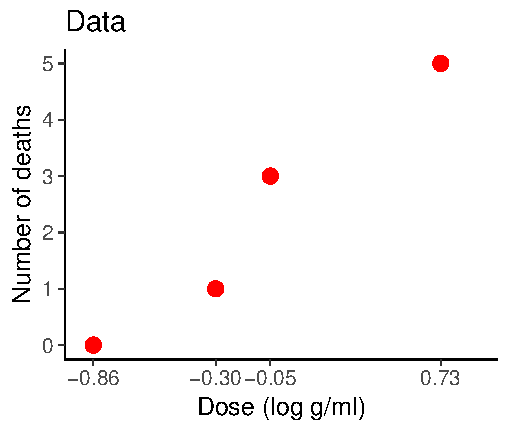
\includegraphics[width=4cm]{figs/bioassay_data_small.pdf}}
  \vspace{2mm}
  \pause

  \vspace{-\baselineskip}
  Find out lethal dose 50\% (LD50)
    \begin{itemize}
      \item[-] used to classify how hazardous chemical is
      \item[-] 1984 EEC directive has 4 levels
      \end{itemize}
  \pause
   Bayesian methods help to
    \begin{itemize}
    \item[-] reduce the number of animals needed
    \item[-] easy to make sequential experiment and stop as soon as
      desired accuracy is obtained
    \end{itemize}
\end{frame}

\begin{frame}{Bioassay}

  \only<1>{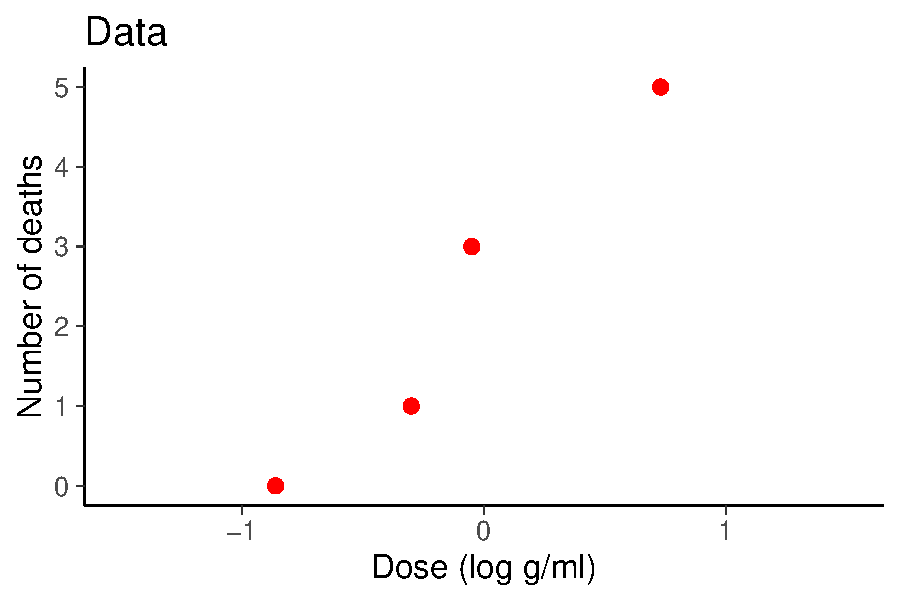
\includegraphics[width=8cm]{figs/bioassay_data.pdf}}
  \only<2>{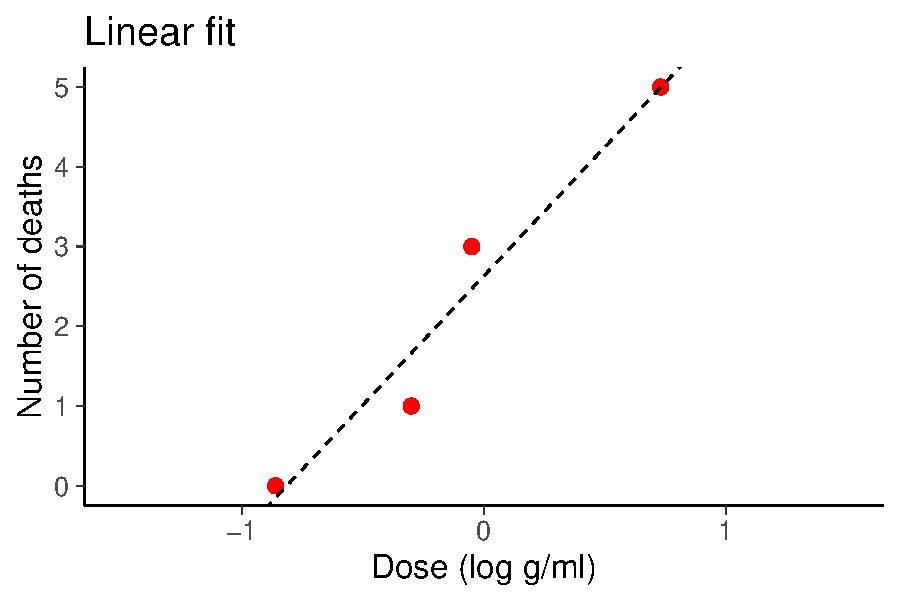
\includegraphics[width=8cm]{figs/bioassay_fitlin.pdf}}
  \only<3>{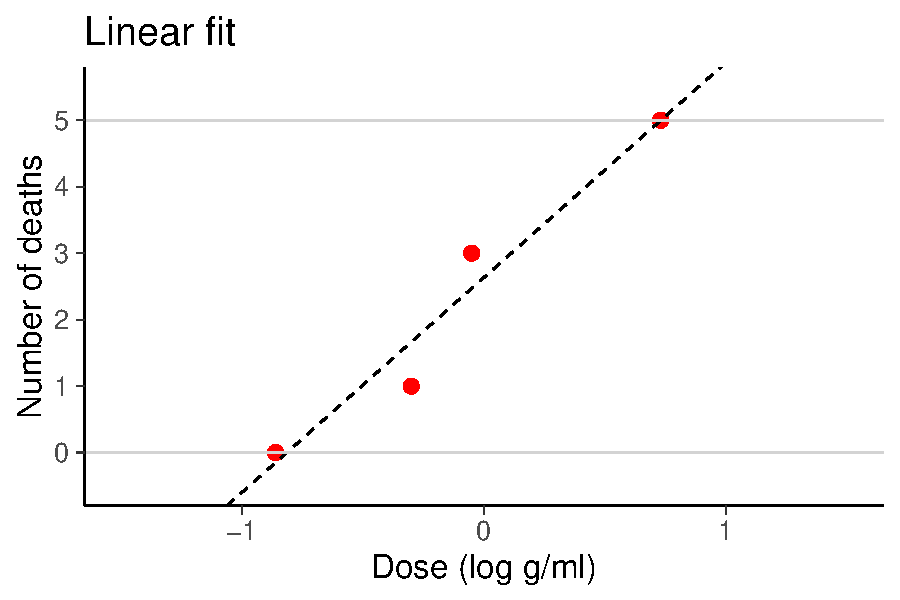
\includegraphics[width=8cm]{figs/bioassay_fitlin2.pdf}}
  \only<4-5>{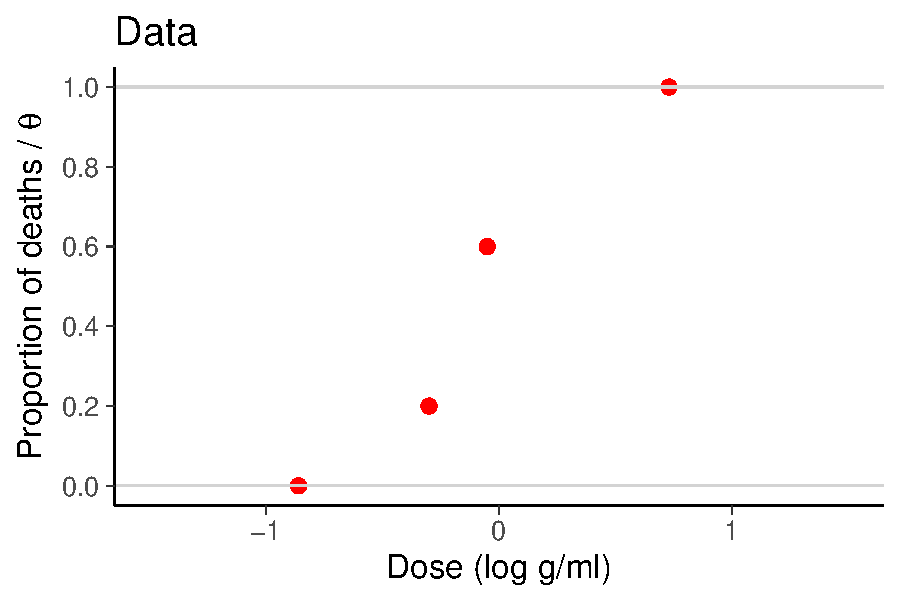
\includegraphics[width=8cm]{figs/bioassay_data2.pdf}\\}
  \only<6>{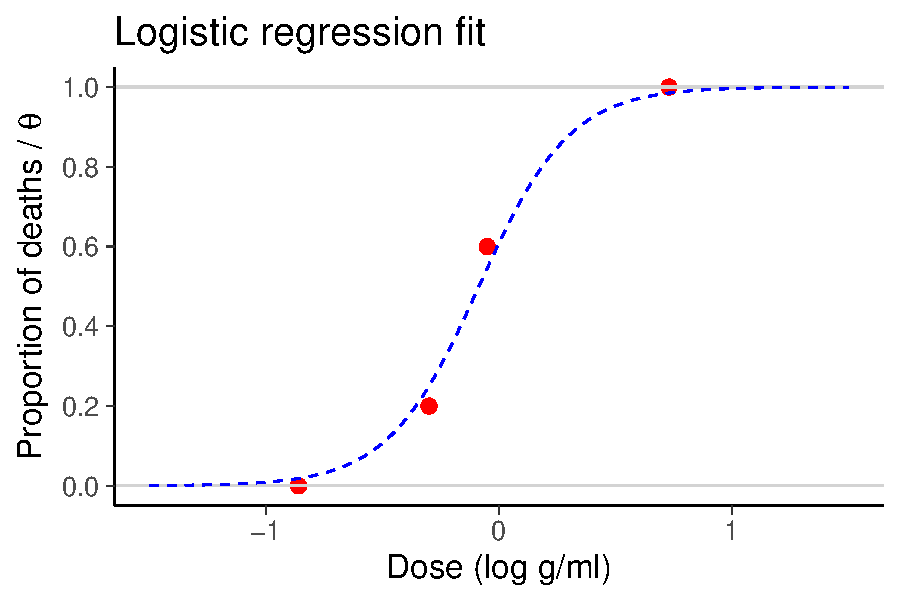
\includegraphics[width=8cm]{figs/bioassay_fitbinom.pdf}\\}
  \only<5->{Binomial model
    \begin{align*}
    y_i \mid {\only<6>{\color{blue}} \theta}_i & \sim \Bin({\only<6>{\color{blue}} \theta}_i,n_i) \uncover<6>{, \quad \logit({\only<6>{\color{blue}}\theta}_i)= \log\left(\frac{{\only<6>{\color{blue}}\theta}_i}{1-{\only<6>{\color{blue}}\theta}_i}\right) = \alpha+\beta x_i}
    \end{align*}
  }

\end{frame}

\begin{frame}{Bioassay}
  \vspace{-0.5\baselineskip}

    \begin{minipage}[b][5cm][t]{4cm}
    \begin{align*}
      y_i \mid \color{blue} \theta_i & \sim \Bin({\color{blue} \theta}_i, n_i)\\
      \logit({\color{blue} \theta}_i) & = \log\left(\frac{{\color{blue} \theta}_i}{1-{\color{blue} \theta}_i}\right)\\
                                     & = {\color{uured} \alpha+\beta x_i} \\
      \uncover<2->{\\ {\color{blue} \theta_i} & = \frac{1}{1+\exp(-({\color{uured}\alpha+\beta x_i}))}}
    \end{align*}
  \end{minipage}~
     \begin{minipage}[b][5cm][t]{4.5cm}
    {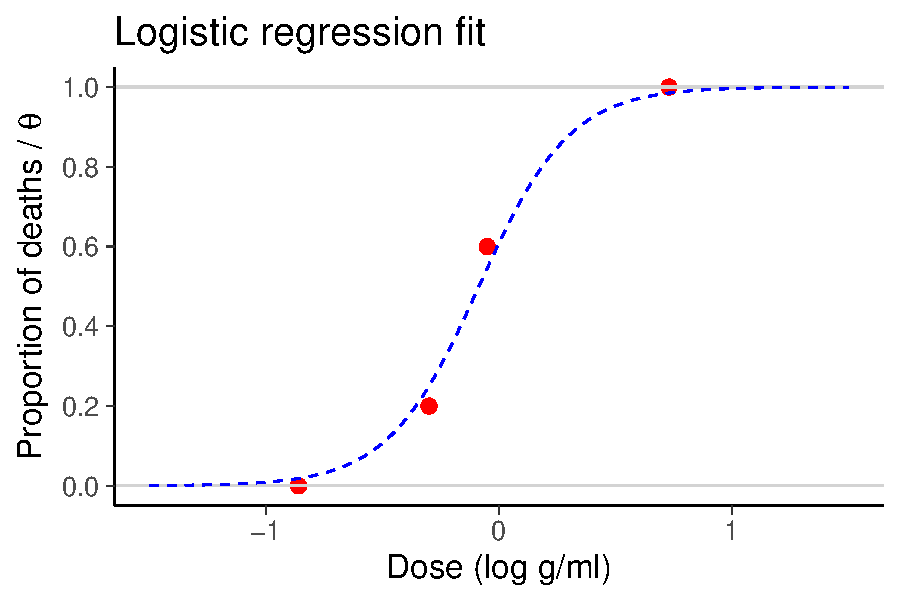
\includegraphics[width=4.5cm]{figs/bioassay_fitbinom.pdf}}
    {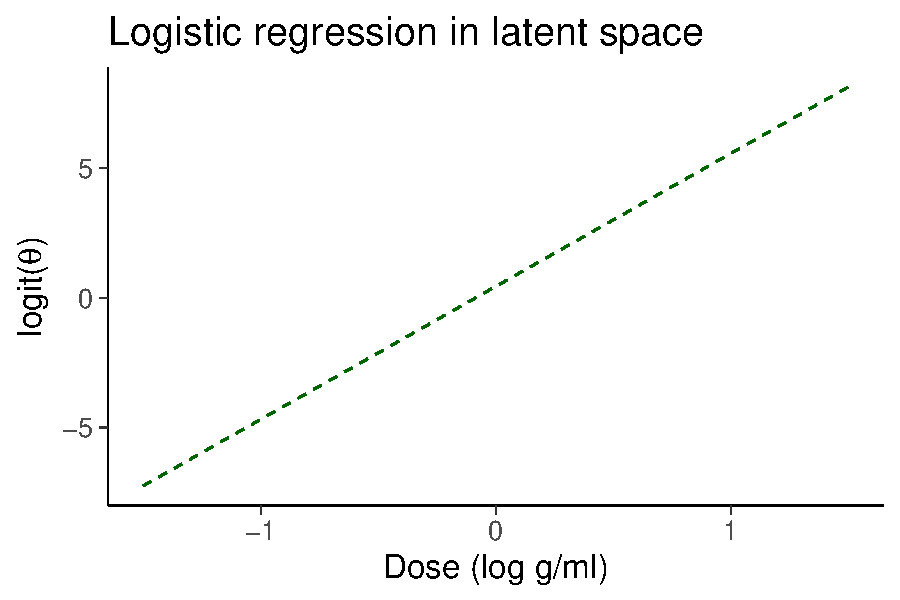
\includegraphics[width=4.5cm]{figs/bioassay_fitlogitspace.pdf}}
  \end{minipage}
\end{frame}

\begin{frame}{Bioassay: Lethal Dose 50\%}

  \only<1>{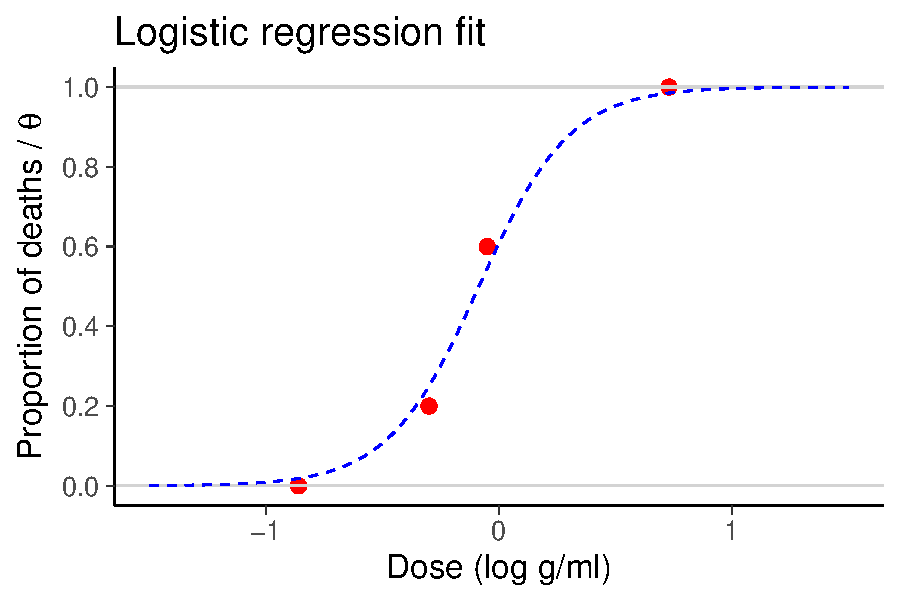
\includegraphics[width=8cm]{figs/bioassay_fitbinom.pdf}}
  \only<2>{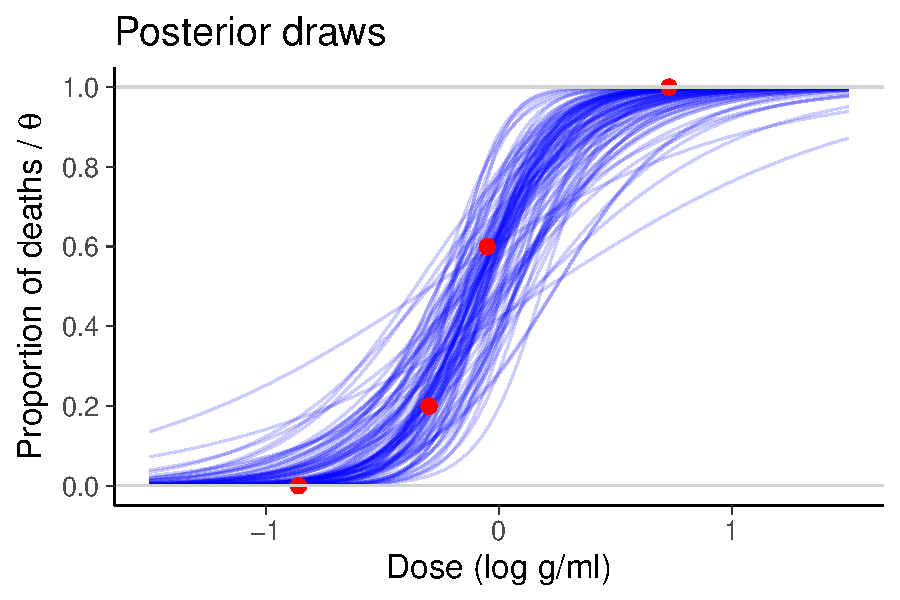
\includegraphics[width=8cm]{figs/bioassay_post.pdf}}
  \only<3-5>{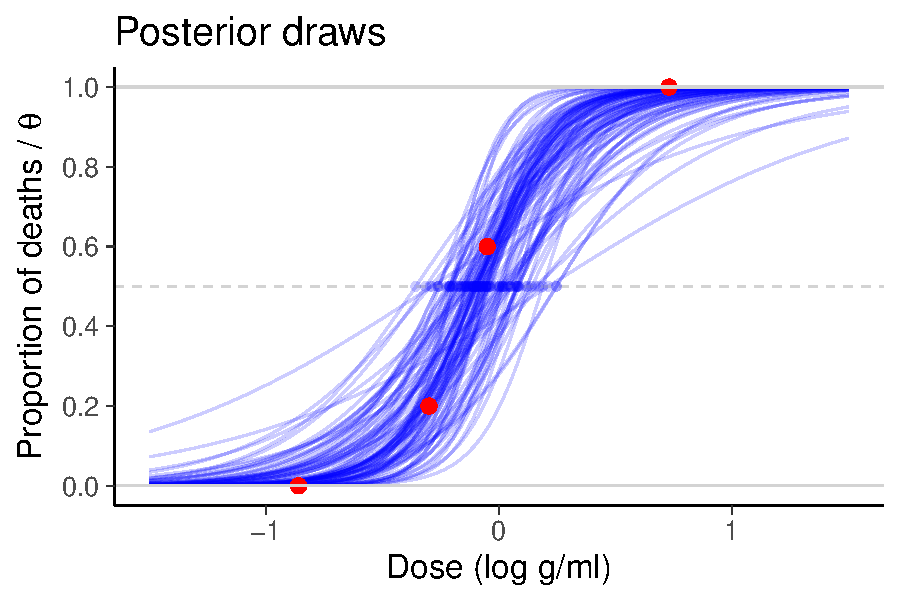
\includegraphics[width=8cm]{figs/bioassay_postld50.pdf}\\}
  \only<6>{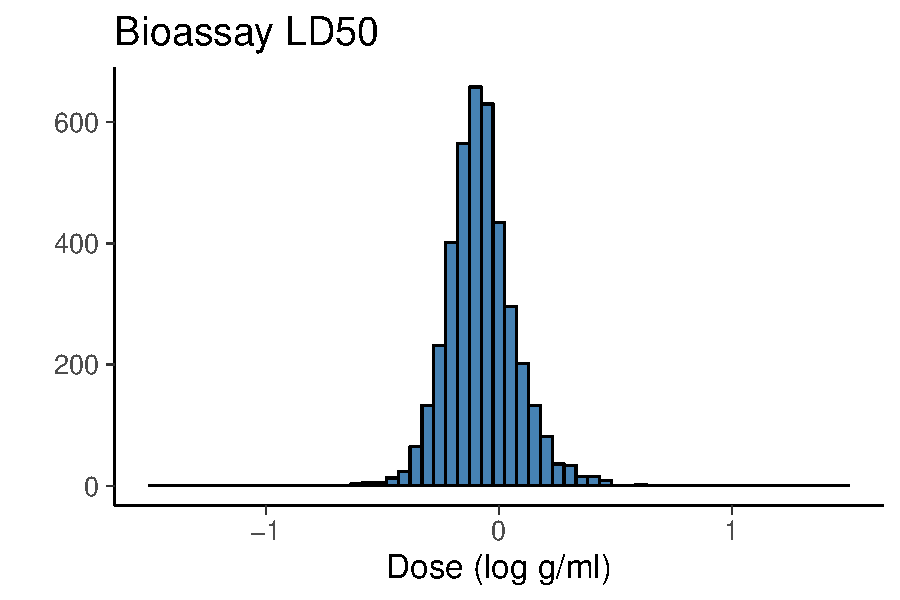
\includegraphics[width=8cm]{figs/bioassay_histld50.pdf}\\}
  \only<3->{
    \vspace{-1.5\baselineskip}
        \begin{align*}
          \E\left(\frac{y}{n}\right)=\logit^{-1}(\alpha+\beta x) = 0.5
          \uncover<4->{\quad \Rightarrow \quad & x_{\mathrm{LD50}}=-\alpha/\beta}\\
          \uncover<5->{& x_{\mathrm{LD50}}^{(s)}=-\alpha^{(s)}/\beta^{(s)}}
    \end{align*}
  }
\end{frame}

\begin{frame}{Bioassay posterior}

  \vspace{-1.5\baselineskip}
    \begin{align*}
      \intertext{Binomial model}
      y_i \mid \theta_i & \sim \Bin(\theta_i,n_i)\\
      \intertext{Link function}
      \logit(\theta_i) & = \alpha+\beta x_i
      \uncover<2->{
  \intertext{Likelihood}
      p(y_i \mid \alpha,\beta,n_i,x_i) & \propto
                                         \theta_i^{y_i}[1-\theta_i]^{n_i-y_i}\\}
      \uncover<3->{
         &  \propto
                                           [\mathrm{logit}^{-1}(\alpha+\beta x_i)]^{y_i}[1-\mathrm{logit}^{-1}(\alpha+\beta x_i)]^{n_i-y_i}\\}
      \uncover<4->{
      \vspace{-1\baselineskip} \\
      \intertext{Posterior}
      p(\alpha,\beta \mid y,n,x) & \propto p(\alpha,\beta)\prod_{i=1}^n p(y_i \mid \alpha,\beta,n_i,x_i)}
      \uncover<4->{
      \vspace{-1\baselineskip} \\
      \intertext{\color{uured} No analytic posterior distribution? What can we do?}
      }
    \end{align*}

\end{frame}

\begin{frame}{Grid evaluation}

\begin{enumerate}
   \item Setup an area (can be hard) for $\alpha$ and $\beta$ that capture most mass (here $\alpha = [-1,5]$ and $\beta = [0,30]$)
   \pause
   \item Compute unnormalized $p(\alpha^{(g)},\beta^{(g)} \mid y,n,x)$, here $\tilde{p}$, at the grid points $g$
   \pause
   \item Sum up $\tilde{p}$ over the whole grid (for all $g \in \{1,...,G\}$)
   \pause
   \item Compute (normalize) the pmf approximation of the posterior $\hat{p}$
\end{enumerate}

\centering
\begin{tabular}{c c c c}
       $g$ & ($\alpha$, $\beta$) & $\tilde{p}$ & $\hat{p}$ \\
      \hline
      1 & (0, -1) & 0.02 & 0.0002 \\
      2 & (0, -0.8) & 0.03 & 0.0003 \\
      ... & ... & ... & ... \\
      G & (30, 5) & 0.001 & 0.00001 \\
      \hline
       $\sum_g^G$ & - & 100 & 1
\end{tabular}

\end{frame}


\begin{frame}{Bioassay (with uniform prior on $\alpha,\beta$)}

  \only<1>{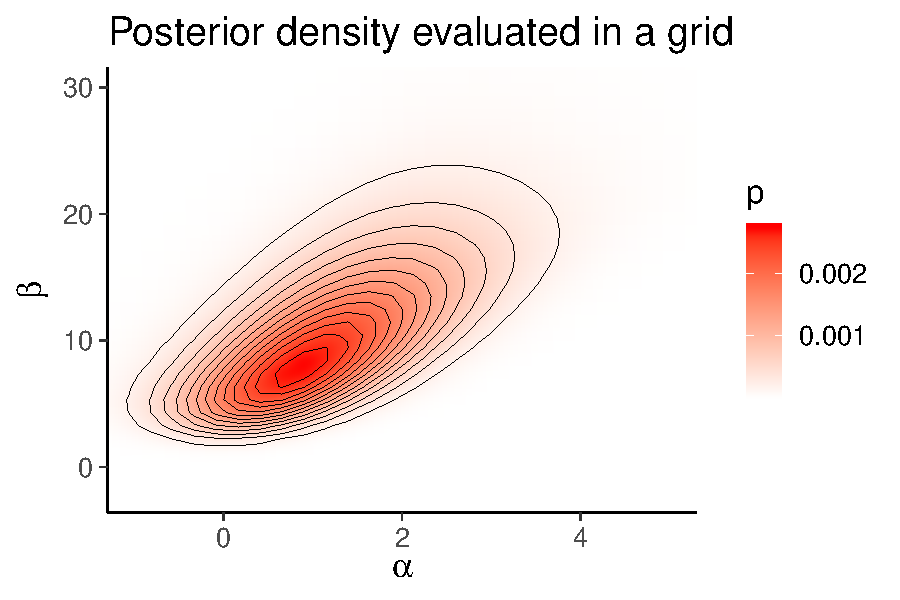
\includegraphics[width=8cm]{figs/bioassay_grid1.pdf}}
  \only<2>{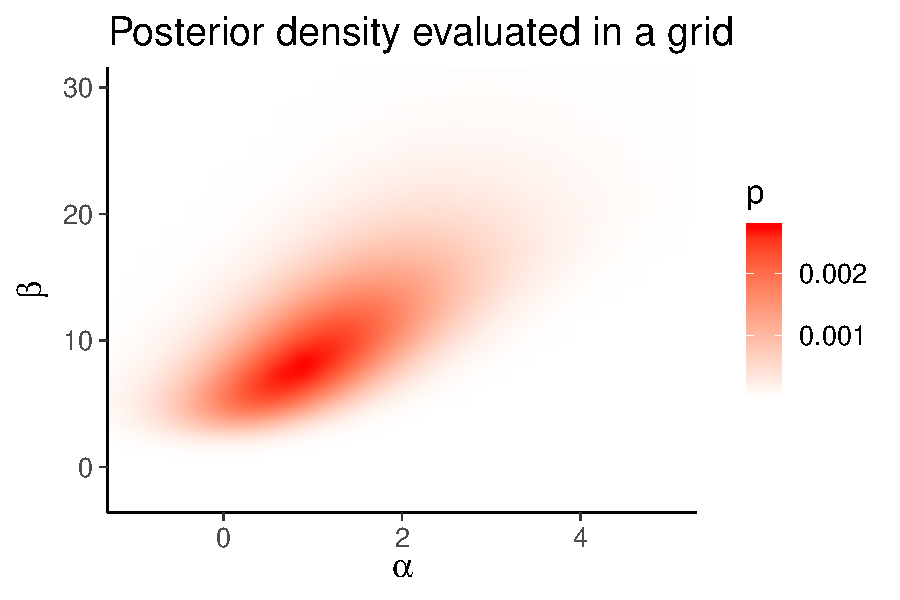
\includegraphics[width=8cm]{figs/bioassay_grid2.pdf}\\
  Density evaluated in grid, but plotted using interpolation}
  \only<3>{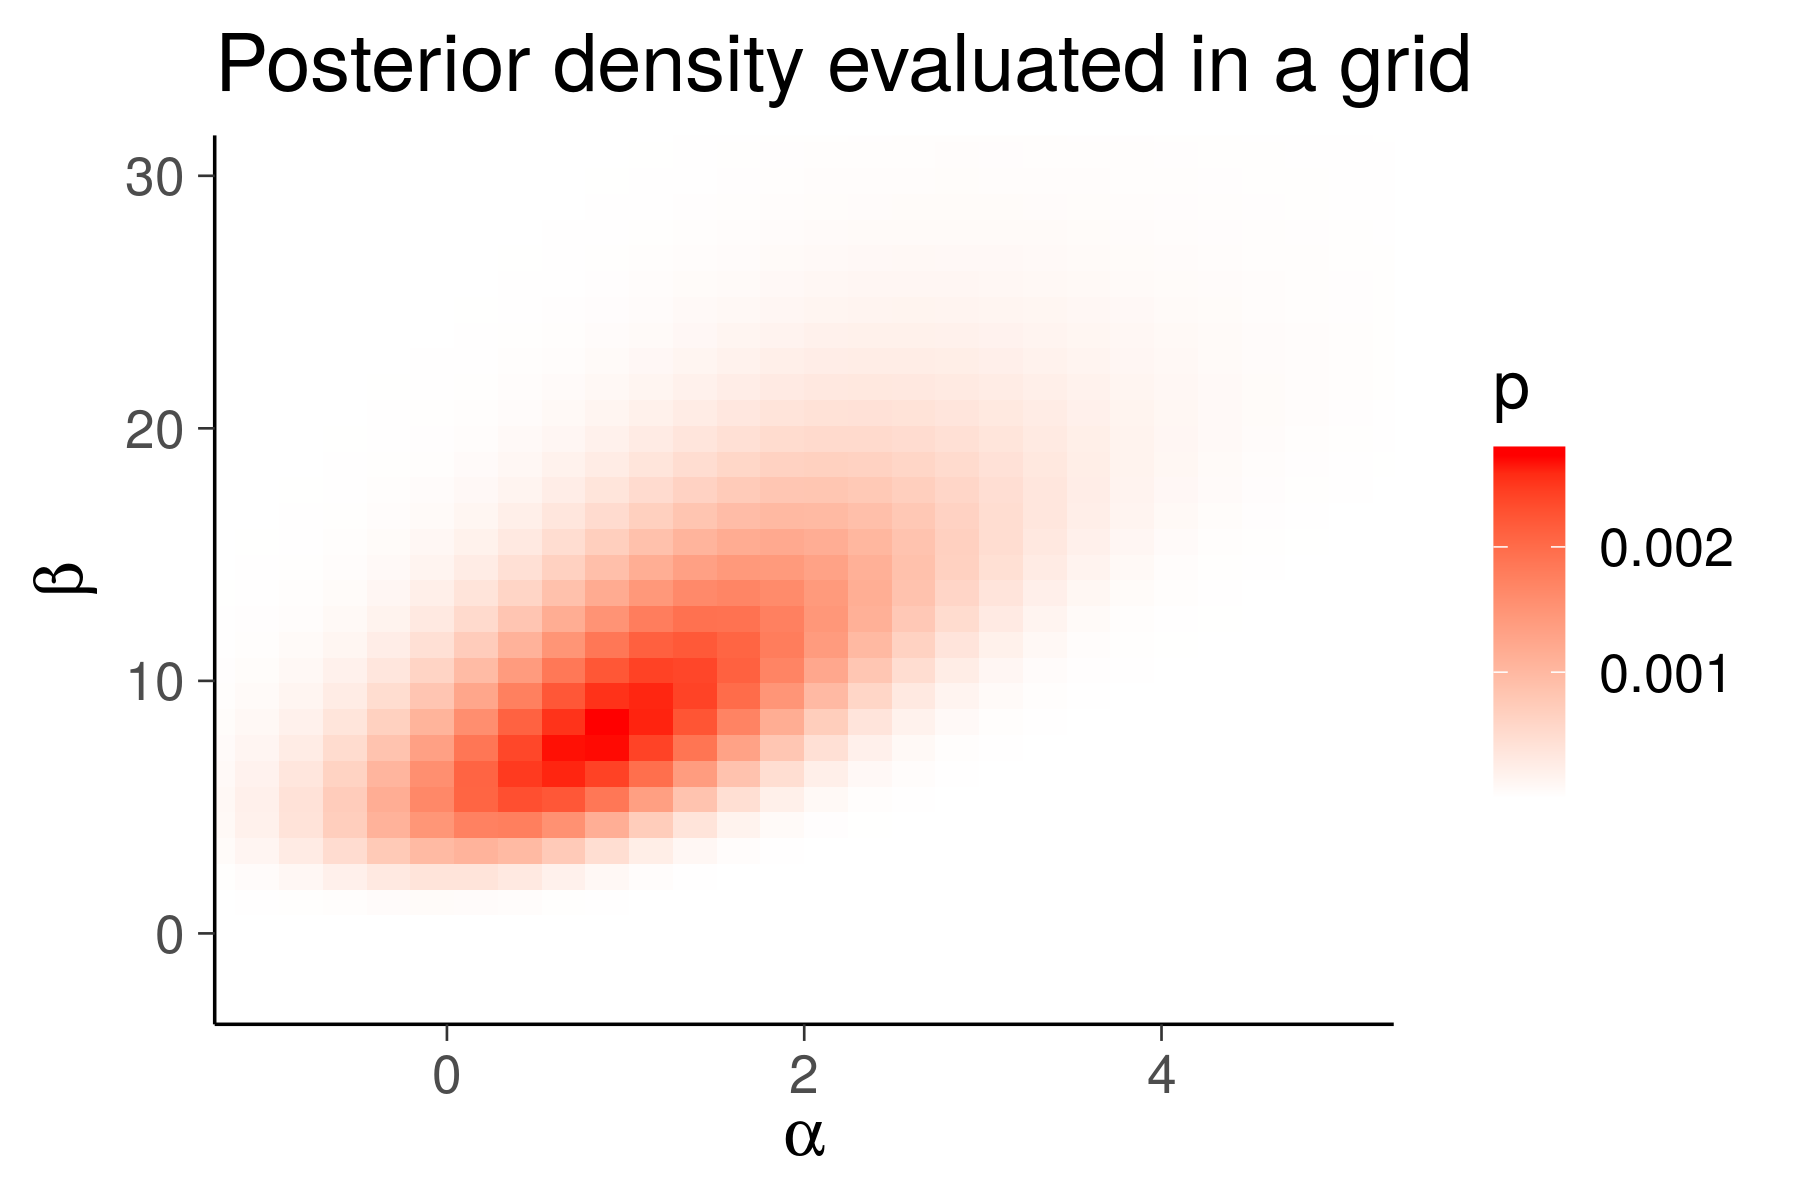
\includegraphics[width=8cm]{figs/bioassay_grid3.png}\\
    Density evaluated in grid, and plotted without interpolation}
  \only<4>{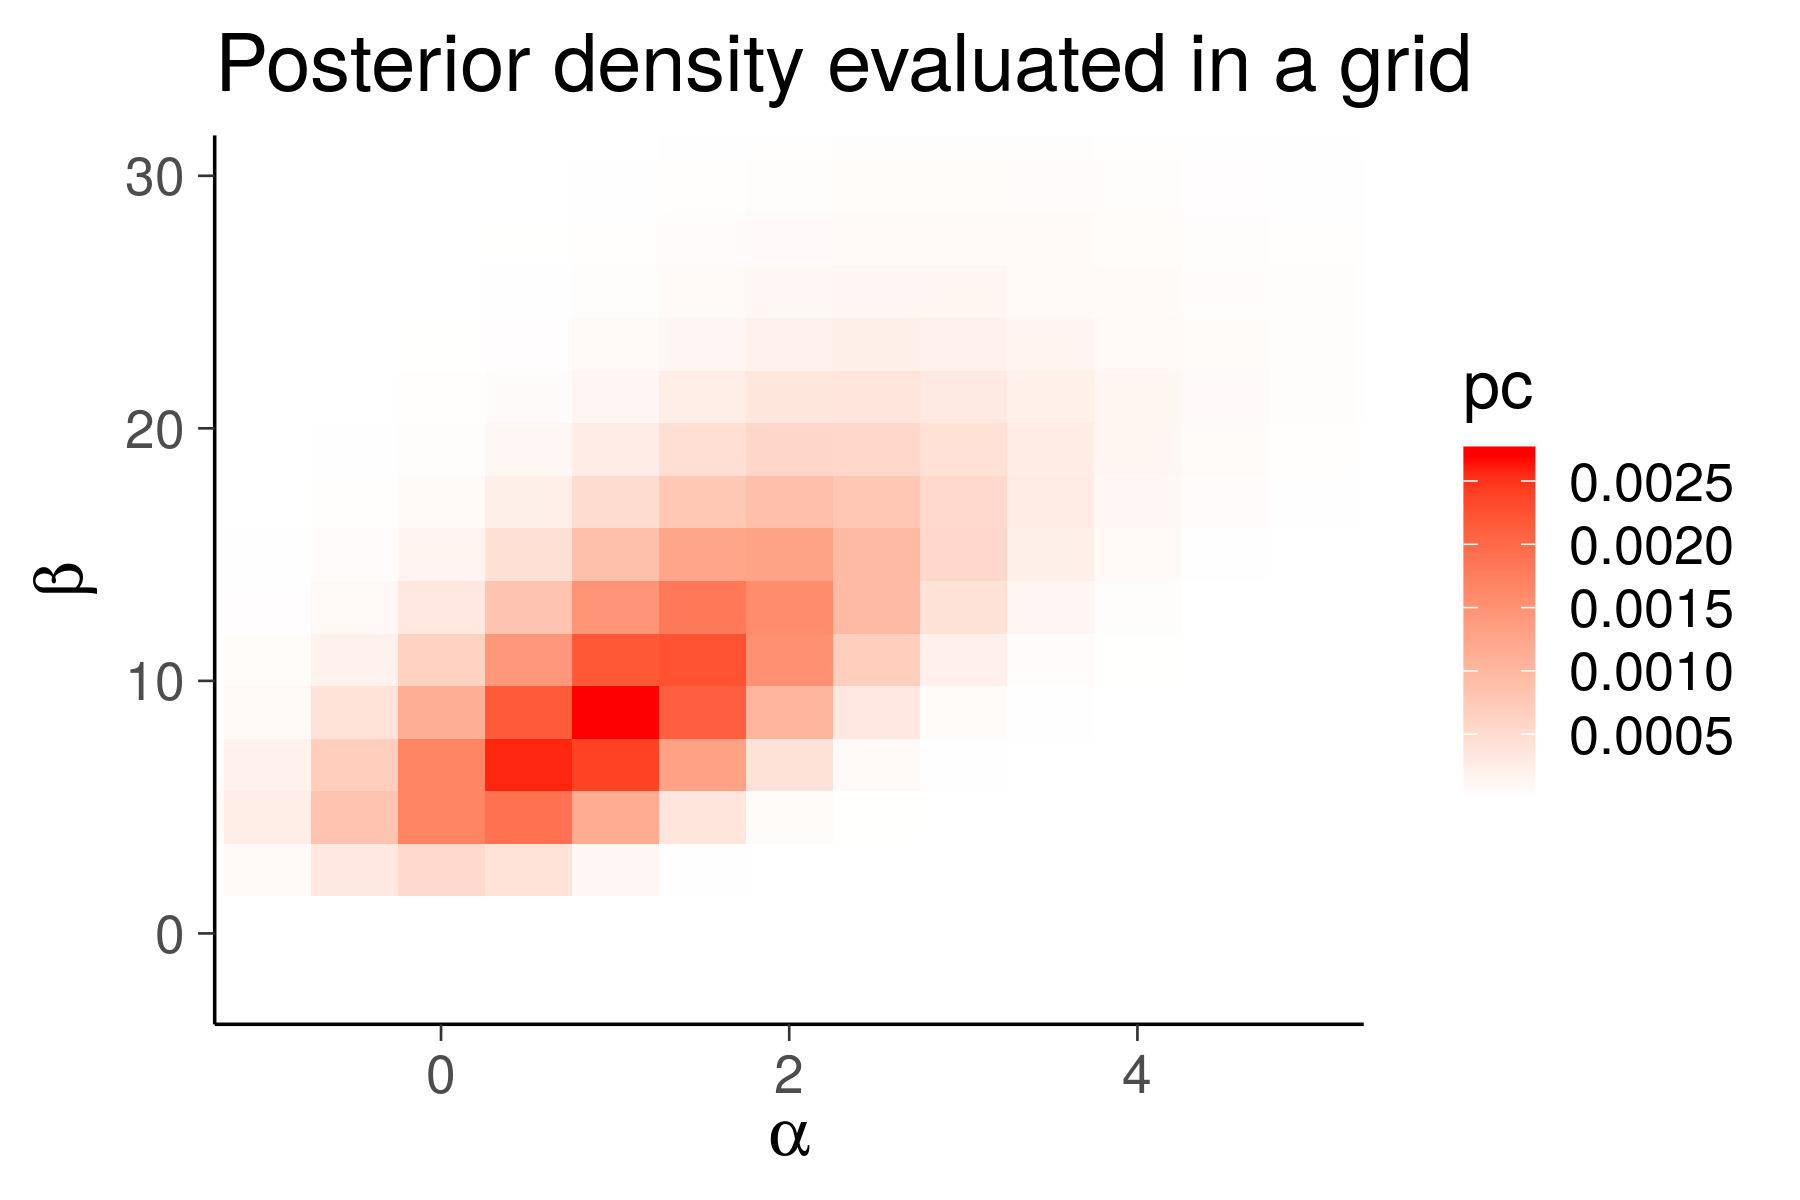
\includegraphics[width=8cm]{figs/bioassay_grid3_1.png} \\
    Density evaluated in a coarser grid}
  \only<5>{\includegraphics[width=8cm]{figs/bioassay_grid3_2.png}\\
    \vspace{-0.5\baselineskip}
    \begin{itemize}
    \item[-] Approximate the density as piecewise constant function
    \item[-] Evaluate density in a grid over some finite region
    \item[-] Density times cell area gives probability mass in each cell
    \end{itemize}
  }
  \only<6>{\includegraphics[width=8cm]{figs/bioassay_grid3_3.png}
    \vspace{-0.5\baselineskip}
    \begin{itemize}
    \item[-] Densities at 1, 2, and 3: 0.0027 0.0010 0.0001
    \item[-] Probabilities of cells 1, 2, and 3: 0.0431 0.0166 0.0010
    \item[-] Probabilities of cells sum to 1
    \end{itemize}
  }
  \only<7>{\includegraphics[width=8cm]{figs/bioassay_grid4.png}\\}
  \only<8>{\includegraphics[width=8cm]{figs/bioassay_grid5.png}\\}
  \only<9>{\includegraphics[width=8cm]{figs/bioassay_grid6.png}\\}
  \only<7-9>{
    \vspace{-0.5\baselineskip}
    \begin{itemize}
    \item[-] Sample according to grid cell probabilities
    \item<9>[-] Several draws can be from the same grid cell
    \end{itemize}
  }
  \only<10>{\includegraphics[width=8cm]{figs/bioassay_grid7.png}\\
    \vspace{-0.5\baselineskip}
    \begin{itemize}
    \item[-] Jitter can be added to improve visualization
    \end{itemize}
  }

\end{frame}


\begin{frame}{Grid sampling}

  \begin{itemize}
  \item[-] Draws can be used to estimate expectations, for example
    \begin{align*}
      E[x_{\mathrm{LD50}}] = E[-\alpha/\beta] & \approx \frac{1}{S}\sum_{s=1}^{S} \frac{\alpha^{(s)}}{\beta^{(s)}}
    \end{align*}
  \item<2->[-] Instead of sampling, grid could be used to evaluate
    functions directly, for example
    \begin{align*}
      \E[-\alpha/\beta] \approx \sum_{t=1}^{T} w_{\mathrm{cell}}^{(t)} \frac{\alpha^{(t)}}{\beta^{(t)}},
    \end{align*}
    where $w_{\mathrm{cell}}^{(t)}$ is the normalized probability of a grid cell $t$, and $\alpha^{(t)}$ and $\beta^{(t)}$ are center locations of grid cells
  \item<3-> Grid sampling gets computationally too expensive in high
    dimensions
  \end{itemize}

\end{frame}



\end{document}



%%%%%%%%%%%%%%%%%%%%%%%%%%%%%%%%%%%%%%%%%%%%%%%%%%%%%%%%%%%%%%%%%%


\end{document}
